% Options for packages loaded elsewhere
\PassOptionsToPackage{unicode}{hyperref}
\PassOptionsToPackage{hyphens}{url}
%
\documentclass[
]{article}
\usepackage{amsmath,amssymb}
\usepackage{lmodern}
\usepackage{iftex}
\ifPDFTeX
  \usepackage[T1]{fontenc}
  \usepackage[utf8]{inputenc}
  \usepackage{textcomp} % provide euro and other symbols
\else % if luatex or xetex
  \usepackage{unicode-math}
  \defaultfontfeatures{Scale=MatchLowercase}
  \defaultfontfeatures[\rmfamily]{Ligatures=TeX,Scale=1}
\fi
% Use upquote if available, for straight quotes in verbatim environments
\IfFileExists{upquote.sty}{\usepackage{upquote}}{}
\IfFileExists{microtype.sty}{% use microtype if available
  \usepackage[]{microtype}
  \UseMicrotypeSet[protrusion]{basicmath} % disable protrusion for tt fonts
}{}
\makeatletter
\@ifundefined{KOMAClassName}{% if non-KOMA class
  \IfFileExists{parskip.sty}{%
    \usepackage{parskip}
  }{% else
    \setlength{\parindent}{0pt}
    \setlength{\parskip}{6pt plus 2pt minus 1pt}}
}{% if KOMA class
  \KOMAoptions{parskip=half}}
\makeatother
\usepackage{xcolor}
\usepackage[margin=1in]{geometry}
\usepackage{color}
\usepackage{fancyvrb}
\newcommand{\VerbBar}{|}
\newcommand{\VERB}{\Verb[commandchars=\\\{\}]}
\DefineVerbatimEnvironment{Highlighting}{Verbatim}{commandchars=\\\{\}}
% Add ',fontsize=\small' for more characters per line
\usepackage{framed}
\definecolor{shadecolor}{RGB}{248,248,248}
\newenvironment{Shaded}{\begin{snugshade}}{\end{snugshade}}
\newcommand{\AlertTok}[1]{\textcolor[rgb]{0.94,0.16,0.16}{#1}}
\newcommand{\AnnotationTok}[1]{\textcolor[rgb]{0.56,0.35,0.01}{\textbf{\textit{#1}}}}
\newcommand{\AttributeTok}[1]{\textcolor[rgb]{0.77,0.63,0.00}{#1}}
\newcommand{\BaseNTok}[1]{\textcolor[rgb]{0.00,0.00,0.81}{#1}}
\newcommand{\BuiltInTok}[1]{#1}
\newcommand{\CharTok}[1]{\textcolor[rgb]{0.31,0.60,0.02}{#1}}
\newcommand{\CommentTok}[1]{\textcolor[rgb]{0.56,0.35,0.01}{\textit{#1}}}
\newcommand{\CommentVarTok}[1]{\textcolor[rgb]{0.56,0.35,0.01}{\textbf{\textit{#1}}}}
\newcommand{\ConstantTok}[1]{\textcolor[rgb]{0.00,0.00,0.00}{#1}}
\newcommand{\ControlFlowTok}[1]{\textcolor[rgb]{0.13,0.29,0.53}{\textbf{#1}}}
\newcommand{\DataTypeTok}[1]{\textcolor[rgb]{0.13,0.29,0.53}{#1}}
\newcommand{\DecValTok}[1]{\textcolor[rgb]{0.00,0.00,0.81}{#1}}
\newcommand{\DocumentationTok}[1]{\textcolor[rgb]{0.56,0.35,0.01}{\textbf{\textit{#1}}}}
\newcommand{\ErrorTok}[1]{\textcolor[rgb]{0.64,0.00,0.00}{\textbf{#1}}}
\newcommand{\ExtensionTok}[1]{#1}
\newcommand{\FloatTok}[1]{\textcolor[rgb]{0.00,0.00,0.81}{#1}}
\newcommand{\FunctionTok}[1]{\textcolor[rgb]{0.00,0.00,0.00}{#1}}
\newcommand{\ImportTok}[1]{#1}
\newcommand{\InformationTok}[1]{\textcolor[rgb]{0.56,0.35,0.01}{\textbf{\textit{#1}}}}
\newcommand{\KeywordTok}[1]{\textcolor[rgb]{0.13,0.29,0.53}{\textbf{#1}}}
\newcommand{\NormalTok}[1]{#1}
\newcommand{\OperatorTok}[1]{\textcolor[rgb]{0.81,0.36,0.00}{\textbf{#1}}}
\newcommand{\OtherTok}[1]{\textcolor[rgb]{0.56,0.35,0.01}{#1}}
\newcommand{\PreprocessorTok}[1]{\textcolor[rgb]{0.56,0.35,0.01}{\textit{#1}}}
\newcommand{\RegionMarkerTok}[1]{#1}
\newcommand{\SpecialCharTok}[1]{\textcolor[rgb]{0.00,0.00,0.00}{#1}}
\newcommand{\SpecialStringTok}[1]{\textcolor[rgb]{0.31,0.60,0.02}{#1}}
\newcommand{\StringTok}[1]{\textcolor[rgb]{0.31,0.60,0.02}{#1}}
\newcommand{\VariableTok}[1]{\textcolor[rgb]{0.00,0.00,0.00}{#1}}
\newcommand{\VerbatimStringTok}[1]{\textcolor[rgb]{0.31,0.60,0.02}{#1}}
\newcommand{\WarningTok}[1]{\textcolor[rgb]{0.56,0.35,0.01}{\textbf{\textit{#1}}}}
\usepackage{graphicx}
\makeatletter
\def\maxwidth{\ifdim\Gin@nat@width>\linewidth\linewidth\else\Gin@nat@width\fi}
\def\maxheight{\ifdim\Gin@nat@height>\textheight\textheight\else\Gin@nat@height\fi}
\makeatother
% Scale images if necessary, so that they will not overflow the page
% margins by default, and it is still possible to overwrite the defaults
% using explicit options in \includegraphics[width, height, ...]{}
\setkeys{Gin}{width=\maxwidth,height=\maxheight,keepaspectratio}
% Set default figure placement to htbp
\makeatletter
\def\fps@figure{htbp}
\makeatother
\setlength{\emergencystretch}{3em} % prevent overfull lines
\providecommand{\tightlist}{%
  \setlength{\itemsep}{0pt}\setlength{\parskip}{0pt}}
\setcounter{secnumdepth}{-\maxdimen} % remove section numbering
\ifLuaTeX
  \usepackage{selnolig}  % disable illegal ligatures
\fi
\IfFileExists{bookmark.sty}{\usepackage{bookmark}}{\usepackage{hyperref}}
\IfFileExists{xurl.sty}{\usepackage{xurl}}{} % add URL line breaks if available
\urlstyle{same} % disable monospaced font for URLs
\hypersetup{
  pdftitle={LongitudinalDataAnalysis},
  pdfauthor={Group2: Wanchang Zhang; Hugo Blain; Oscar Cabanelas},
  hidelinks,
  pdfcreator={LaTeX via pandoc}}

\title{LongitudinalDataAnalysis}
\author{Group2: Wanchang Zhang; Hugo Blain; Oscar Cabanelas}
\date{2023-03-05}

\begin{document}
\maketitle

\hypertarget{introduction}{%
\section{0. Introduction}\label{introduction}}

The dataset contains information on patients who received renal
graft(kidney transplant) The patients have been followed for at most 10
years.

Background: People with end-stage kidney disease who receive a kidney
transplant generally live longer than people with ESRD who are on
dialysis.

However, kidney transplant recipients must remain on immunosuppressants
(medications to suppress the immune system) for the rest of their life
to prevent their body from rejecting the new kidney. The long-term
immunosuppression puts them at risk for infections and cancer.

The Haermatocrit level (HC level) usually differs with gender, Also the
health condition of a person.

\hypertarget{task-for-week-one}{%
\section{1. Task for week one}\label{task-for-week-one}}

\hypertarget{import-data}{%
\subsection{1.1 Import data}\label{import-data}}

\begin{Shaded}
\begin{Highlighting}[]
\CommentTok{\#install.packages("readxl")}
\FunctionTok{library}\NormalTok{(readxl)}
\NormalTok{trenal }\OtherTok{\textless{}{-}} \FunctionTok{read\_excel}\NormalTok{(}\StringTok{"Trenal.XLS"}\NormalTok{)}
\FunctionTok{summary}\NormalTok{(trenal)}
\end{Highlighting}
\end{Shaded}

\begin{verbatim}
##       HC0             HC06            HC1             HC2            HC3       
##  Min.   :14.00   Min.   :22.00   Min.   :20.00   Min.   :17.0   Min.   :20.00  
##  1st Qu.:28.00   1st Qu.:35.00   1st Qu.:36.00   1st Qu.:36.0   1st Qu.:36.00  
##  Median :32.00   Median :38.55   Median :39.00   Median :40.0   Median :39.00  
##  Mean   :31.86   Mean   :38.83   Mean   :39.71   Mean   :39.7   Mean   :39.17  
##  3rd Qu.:36.00   3rd Qu.:42.00   3rd Qu.:43.00   3rd Qu.:43.0   3rd Qu.:43.00  
##  Max.   :60.00   Max.   :61.70   Max.   :63.00   Max.   :65.0   Max.   :60.00  
##  NA's   :12                      NA's   :12      NA's   :1044   NA's   :2460   
##       HC4             HC5             HC6             HC7       
##  Min.   :23.00   Min.   :17.00   Min.   :20.00   Min.   :17.00  
##  1st Qu.:35.00   1st Qu.:35.00   1st Qu.:36.00   1st Qu.:35.00  
##  Median :39.00   Median :39.00   Median :39.00   Median :39.00  
##  Mean   :39.16   Mean   :39.02   Mean   :39.11   Mean   :38.85  
##  3rd Qu.:43.00   3rd Qu.:43.00   3rd Qu.:43.00   3rd Qu.:42.00  
##  Max.   :55.00   Max.   :56.00   Max.   :55.00   Max.   :60.00  
##  NA's   :3768    NA's   :5016    NA's   :6096    NA's   :7140   
##       HC8             HC9             HC10             id        
##  Min.   :23.00   Min.   :17.00   Min.   :24.10   Min.   :   1.0  
##  1st Qu.:35.00   1st Qu.:35.00   1st Qu.:35.00   1st Qu.: 290.8  
##  Median :38.05   Median :38.50   Median :38.00   Median : 580.5  
##  Mean   :38.35   Mean   :38.57   Mean   :38.49   Mean   : 580.5  
##  3rd Qu.:42.00   3rd Qu.:42.00   3rd Qu.:42.00   3rd Qu.: 870.2  
##  Max.   :55.00   Max.   :55.00   Max.   :54.00   Max.   :1160.0  
##  NA's   :8064    NA's   :8988    NA's   :9744                    
##       age             male            cardio           reject           const  
##  Min.   :15.00   Min.   :0.0000   Min.   :0.0000   Min.   :0.0000   Min.   :1  
##  1st Qu.:36.00   1st Qu.:0.0000   1st Qu.:0.0000   1st Qu.:0.0000   1st Qu.:1  
##  Median :48.00   Median :1.0000   Median :0.0000   Median :0.0000   Median :1  
##  Mean   :46.43   Mean   :0.5741   Mean   :0.1784   Mean   :0.3164   Mean   :1  
##  3rd Qu.:57.00   3rd Qu.:1.0000   3rd Qu.:0.0000   3rd Qu.:1.0000   3rd Qu.:1  
##  Max.   :76.00   Max.   :1.0000   Max.   :1.0000   Max.   :1.0000   Max.   :1  
##  NA's   :12                                                                    
##        j            respons           time       
##  Min.   : 1.00   Min.   :14.00   Min.   : 0.000  
##  1st Qu.: 3.75   1st Qu.:34.00   1st Qu.: 1.750  
##  Median : 6.50   Median :38.00   Median : 4.500  
##  Mean   : 6.50   Mean   :38.24   Mean   : 4.625  
##  3rd Qu.: 9.25   3rd Qu.:42.00   3rd Qu.: 7.250  
##  Max.   :12.00   Max.   :65.00   Max.   :10.000  
##                  NA's   :4362
\end{verbatim}

remove a noninformative column const

\begin{Shaded}
\begin{Highlighting}[]
\NormalTok{trenal}\OtherTok{=}\NormalTok{ trenal[,}\SpecialCharTok{{-}}\DecValTok{18}\NormalTok{]}
\FunctionTok{summary}\NormalTok{(trenal)}
\end{Highlighting}
\end{Shaded}

\begin{verbatim}
##       HC0             HC06            HC1             HC2            HC3       
##  Min.   :14.00   Min.   :22.00   Min.   :20.00   Min.   :17.0   Min.   :20.00  
##  1st Qu.:28.00   1st Qu.:35.00   1st Qu.:36.00   1st Qu.:36.0   1st Qu.:36.00  
##  Median :32.00   Median :38.55   Median :39.00   Median :40.0   Median :39.00  
##  Mean   :31.86   Mean   :38.83   Mean   :39.71   Mean   :39.7   Mean   :39.17  
##  3rd Qu.:36.00   3rd Qu.:42.00   3rd Qu.:43.00   3rd Qu.:43.0   3rd Qu.:43.00  
##  Max.   :60.00   Max.   :61.70   Max.   :63.00   Max.   :65.0   Max.   :60.00  
##  NA's   :12                      NA's   :12      NA's   :1044   NA's   :2460   
##       HC4             HC5             HC6             HC7       
##  Min.   :23.00   Min.   :17.00   Min.   :20.00   Min.   :17.00  
##  1st Qu.:35.00   1st Qu.:35.00   1st Qu.:36.00   1st Qu.:35.00  
##  Median :39.00   Median :39.00   Median :39.00   Median :39.00  
##  Mean   :39.16   Mean   :39.02   Mean   :39.11   Mean   :38.85  
##  3rd Qu.:43.00   3rd Qu.:43.00   3rd Qu.:43.00   3rd Qu.:42.00  
##  Max.   :55.00   Max.   :56.00   Max.   :55.00   Max.   :60.00  
##  NA's   :3768    NA's   :5016    NA's   :6096    NA's   :7140   
##       HC8             HC9             HC10             id        
##  Min.   :23.00   Min.   :17.00   Min.   :24.10   Min.   :   1.0  
##  1st Qu.:35.00   1st Qu.:35.00   1st Qu.:35.00   1st Qu.: 290.8  
##  Median :38.05   Median :38.50   Median :38.00   Median : 580.5  
##  Mean   :38.35   Mean   :38.57   Mean   :38.49   Mean   : 580.5  
##  3rd Qu.:42.00   3rd Qu.:42.00   3rd Qu.:42.00   3rd Qu.: 870.2  
##  Max.   :55.00   Max.   :55.00   Max.   :54.00   Max.   :1160.0  
##  NA's   :8064    NA's   :8988    NA's   :9744                    
##       age             male            cardio           reject      
##  Min.   :15.00   Min.   :0.0000   Min.   :0.0000   Min.   :0.0000  
##  1st Qu.:36.00   1st Qu.:0.0000   1st Qu.:0.0000   1st Qu.:0.0000  
##  Median :48.00   Median :1.0000   Median :0.0000   Median :0.0000  
##  Mean   :46.43   Mean   :0.5741   Mean   :0.1784   Mean   :0.3164  
##  3rd Qu.:57.00   3rd Qu.:1.0000   3rd Qu.:0.0000   3rd Qu.:1.0000  
##  Max.   :76.00   Max.   :1.0000   Max.   :1.0000   Max.   :1.0000  
##  NA's   :12                                                        
##        j            respons           time       
##  Min.   : 1.00   Min.   :14.00   Min.   : 0.000  
##  1st Qu.: 3.75   1st Qu.:34.00   1st Qu.: 1.750  
##  Median : 6.50   Median :38.00   Median : 4.500  
##  Mean   : 6.50   Mean   :38.24   Mean   : 4.625  
##  3rd Qu.: 9.25   3rd Qu.:42.00   3rd Qu.: 7.250  
##  Max.   :12.00   Max.   :65.00   Max.   :10.000  
##                  NA's   :4362
\end{verbatim}

\begin{Shaded}
\begin{Highlighting}[]
\FunctionTok{dim}\NormalTok{(trenal)}
\end{Highlighting}
\end{Shaded}

\begin{verbatim}
## [1] 13920    20
\end{verbatim}

\hypertarget{table-structure-analysis-and-variable-understanding}{%
\subsection{1.2 Table structure analysis and variable
understanding}\label{table-structure-analysis-and-variable-understanding}}

The table contains observation of HC level on 1160 patients who have
gone through kidney transplant. Each patient will have maximum 12
meassurements in the 12 time point \((0,0.5,1,2,\cdots,10)\) years.

if we just look at the first 12 columns, they are all Haematocrit level
at the corresponding time. Thus our response variable is Haematocrit
level. If we just look at first 17 columns from HC0 to reject, then the
subtable looks like a wide table; If we start from column id to column
time, the part of table is a long table. From now on we focus on the
long table:

\begin{Shaded}
\begin{Highlighting}[]
\NormalTok{trenal.long }\OtherTok{=}\NormalTok{ trenal[,}\DecValTok{13}\SpecialCharTok{:}\DecValTok{20}\NormalTok{]}
\FunctionTok{summary}\NormalTok{(trenal.long)}
\end{Highlighting}
\end{Shaded}

\begin{verbatim}
##        id              age             male            cardio      
##  Min.   :   1.0   Min.   :15.00   Min.   :0.0000   Min.   :0.0000  
##  1st Qu.: 290.8   1st Qu.:36.00   1st Qu.:0.0000   1st Qu.:0.0000  
##  Median : 580.5   Median :48.00   Median :1.0000   Median :0.0000  
##  Mean   : 580.5   Mean   :46.43   Mean   :0.5741   Mean   :0.1784  
##  3rd Qu.: 870.2   3rd Qu.:57.00   3rd Qu.:1.0000   3rd Qu.:0.0000  
##  Max.   :1160.0   Max.   :76.00   Max.   :1.0000   Max.   :1.0000  
##                   NA's   :12                                       
##      reject             j            respons           time       
##  Min.   :0.0000   Min.   : 1.00   Min.   :14.00   Min.   : 0.000  
##  1st Qu.:0.0000   1st Qu.: 3.75   1st Qu.:34.00   1st Qu.: 1.750  
##  Median :0.0000   Median : 6.50   Median :38.00   Median : 4.500  
##  Mean   :0.3164   Mean   : 6.50   Mean   :38.24   Mean   : 4.625  
##  3rd Qu.:1.0000   3rd Qu.: 9.25   3rd Qu.:42.00   3rd Qu.: 7.250  
##  Max.   :1.0000   Max.   :12.00   Max.   :65.00   Max.   :10.000  
##                                   NA's   :4362
\end{verbatim}

\begin{Shaded}
\begin{Highlighting}[]
\FunctionTok{dim}\NormalTok{(trenal.long)}
\end{Highlighting}
\end{Shaded}

\begin{verbatim}
## [1] 13920     8
\end{verbatim}

Besides the time \(0,0.5,1,2,3,4,5,\cdots,10\) is one-to-one
correspondent to j \(1,2,3,\cdots,12\). But we can still leave it in the
dataframe. Our response variable is the HC level(The percentage of red
cells in the blood, normal levels of hermatocrit for men range from
\(41\%\) to \(50\%\), normal level for women is \(36\%\) to \(48\%\))
the explanatory variables are age, we can change the structure of the
table as we are used to: Identity, time, respons, explanatory variables
(time dependent), explanatory variables (time independent). The response
variables are some continuous integer values? The explanatory variables
have binary type: male, cardio, reject, and integer type: age

\begin{Shaded}
\begin{Highlighting}[]
\CommentTok{\#install.packages("magrittr") \# package installations are only needed the first time you use it}
\CommentTok{\#install.packages("dplyr")    \# alternative installation of the \%\textgreater{}\%}
\FunctionTok{library}\NormalTok{(magrittr) }\CommentTok{\# needs to be run every time you start R and want to use \%\textgreater{}\%}
\FunctionTok{library}\NormalTok{(dplyr)   }
\end{Highlighting}
\end{Shaded}

\begin{verbatim}
## 
## Attaching package: 'dplyr'
\end{verbatim}

\begin{verbatim}
## The following objects are masked from 'package:stats':
## 
##     filter, lag
\end{verbatim}

\begin{verbatim}
## The following objects are masked from 'package:base':
## 
##     intersect, setdiff, setequal, union
\end{verbatim}

\begin{Shaded}
\begin{Highlighting}[]
\NormalTok{data }\OtherTok{\textless{}{-}}\NormalTok{ trenal.long }\SpecialCharTok{\%\textgreater{}\%} 
  \FunctionTok{relocate}\NormalTok{(id) }\SpecialCharTok{\%\textgreater{}\%}
  \FunctionTok{relocate}\NormalTok{(j,}\AttributeTok{.after=}\NormalTok{id)}\SpecialCharTok{\%\textgreater{}\%}
  \FunctionTok{relocate}\NormalTok{(time,}\AttributeTok{.after =}\NormalTok{ j)}\SpecialCharTok{\%\textgreater{}\%}
  \FunctionTok{relocate}\NormalTok{(respons,}\AttributeTok{.after=}\NormalTok{time)}
\NormalTok{trenal.long}\SpecialCharTok{$}\NormalTok{id }\OtherTok{=} \FunctionTok{as.factor}\NormalTok{(trenal.long}\SpecialCharTok{$}\NormalTok{id)}
\NormalTok{trenal.long}\SpecialCharTok{$}\NormalTok{j }\OtherTok{=} \FunctionTok{as.factor}\NormalTok{(trenal.long}\SpecialCharTok{$}\NormalTok{j)}
\NormalTok{trenal.long}\SpecialCharTok{$}\NormalTok{male }\OtherTok{=} \FunctionTok{as.factor}\NormalTok{(trenal.long}\SpecialCharTok{$}\NormalTok{male)}
\NormalTok{trenal.long}\SpecialCharTok{$}\NormalTok{cardio }\OtherTok{=} \FunctionTok{as.factor}\NormalTok{(trenal.long}\SpecialCharTok{$}\NormalTok{cardio)}
\NormalTok{trenal.long}\SpecialCharTok{$}\NormalTok{reject }\OtherTok{=} \FunctionTok{as.factor}\NormalTok{(trenal.long}\SpecialCharTok{$}\NormalTok{reject)}
\FunctionTok{summary}\NormalTok{(trenal.long)}
\end{Highlighting}
\end{Shaded}

\begin{verbatim}
##        id             age        male     cardio    reject         j       
##  1      :   12   Min.   :15.00   0:5928   0:11436   0:9516   1      :1160  
##  2      :   12   1st Qu.:36.00   1:7992   1: 2484   1:4404   2      :1160  
##  3      :   12   Median :48.00                               3      :1160  
##  4      :   12   Mean   :46.43                               4      :1160  
##  5      :   12   3rd Qu.:57.00                               5      :1160  
##  6      :   12   Max.   :76.00                               6      :1160  
##  (Other):13848   NA's   :12                                  (Other):6960  
##     respons           time       
##  Min.   :14.00   Min.   : 0.000  
##  1st Qu.:34.00   1st Qu.: 1.750  
##  Median :38.00   Median : 4.500  
##  Mean   :38.24   Mean   : 4.625  
##  3rd Qu.:42.00   3rd Qu.: 7.250  
##  Max.   :65.00   Max.   :10.000  
##  NA's   :4362
\end{verbatim}

\begin{Shaded}
\begin{Highlighting}[]
\FunctionTok{length}\NormalTok{(}\FunctionTok{unique}\NormalTok{(trenal.long}\SpecialCharTok{$}\NormalTok{id))}
\end{Highlighting}
\end{Shaded}

\begin{verbatim}
## [1] 1160
\end{verbatim}

\begin{Shaded}
\begin{Highlighting}[]
\CommentTok{\# Plot the raw data}
\CommentTok{\#install.packages("tigerstats") }
\FunctionTok{require}\NormalTok{(tigerstats)}
\end{Highlighting}
\end{Shaded}

\begin{verbatim}
## Loading required package: tigerstats
\end{verbatim}

\begin{verbatim}
## Loading required package: abd
\end{verbatim}

\begin{verbatim}
## Loading required package: nlme
\end{verbatim}

\begin{verbatim}
## 
## Attaching package: 'nlme'
\end{verbatim}

\begin{verbatim}
## The following object is masked from 'package:dplyr':
## 
##     collapse
\end{verbatim}

\begin{verbatim}
## Loading required package: lattice
\end{verbatim}

\begin{verbatim}
## Loading required package: grid
\end{verbatim}

\begin{verbatim}
## Loading required package: mosaic
\end{verbatim}

\begin{verbatim}
## Registered S3 method overwritten by 'mosaic':
##   method                           from   
##   fortify.SpatialPolygonsDataFrame ggplot2
\end{verbatim}

\begin{verbatim}
## 
## The 'mosaic' package masks several functions from core packages in order to add 
## additional features.  The original behavior of these functions should not be affected by this.
\end{verbatim}

\begin{verbatim}
## 
## Attaching package: 'mosaic'
\end{verbatim}

\begin{verbatim}
## The following object is masked from 'package:Matrix':
## 
##     mean
\end{verbatim}

\begin{verbatim}
## The following object is masked from 'package:ggplot2':
## 
##     stat
\end{verbatim}

\begin{verbatim}
## The following objects are masked from 'package:dplyr':
## 
##     count, do, tally
\end{verbatim}

\begin{verbatim}
## The following objects are masked from 'package:stats':
## 
##     binom.test, cor, cor.test, cov, fivenum, IQR, median, prop.test,
##     quantile, sd, t.test, var
\end{verbatim}

\begin{verbatim}
## The following objects are masked from 'package:base':
## 
##     max, mean, min, prod, range, sample, sum
\end{verbatim}

\begin{verbatim}
## Welcome to tigerstats!
## To learn more about this package, consult its website:
##  http://homerhanumat.github.io/tigerstats
\end{verbatim}

\begin{Shaded}
\begin{Highlighting}[]
\FunctionTok{xyplot}\NormalTok{(respons }\SpecialCharTok{\textasciitilde{}}\NormalTok{ time, }\AttributeTok{groups =}\NormalTok{ id, }\AttributeTok{data=}\NormalTok{data, }\AttributeTok{type=}\StringTok{"l"}\NormalTok{,}\AttributeTok{xlab=}\StringTok{"Time (year)"}\NormalTok{,}\AttributeTok{ylab=}\StringTok{"HC level "}\NormalTok{ )}
\end{Highlighting}
\end{Shaded}

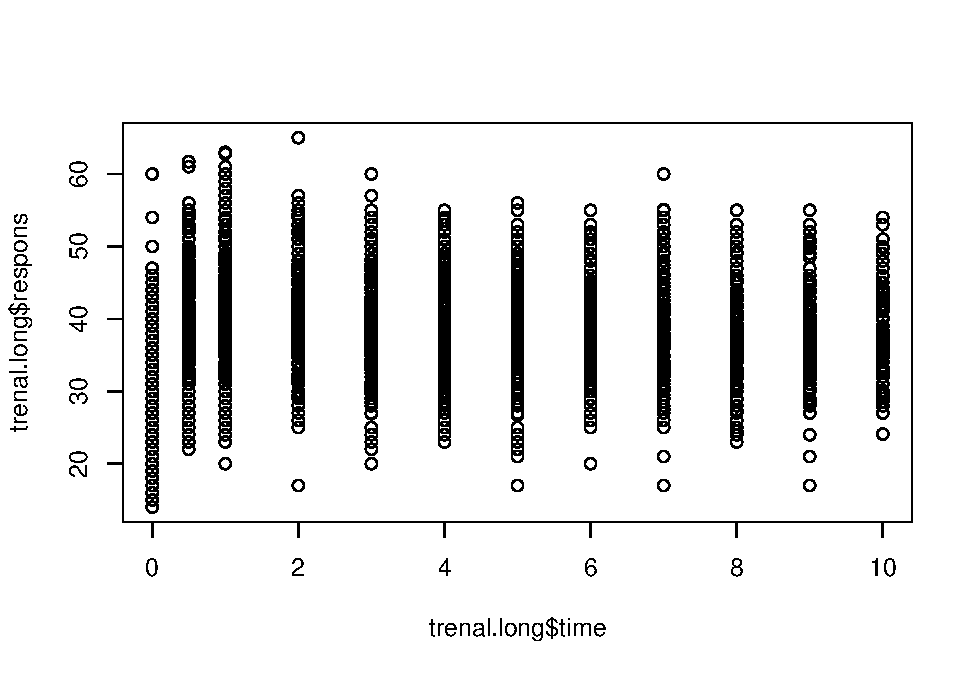
\includegraphics{LDA_Wan_files/figure-latex/unnamed-chunk-7-1.pdf}

\begin{Shaded}
\begin{Highlighting}[]
\FunctionTok{library}\NormalTok{(ggplot2)}
\FunctionTok{library}\NormalTok{(nlme)}
\FunctionTok{library}\NormalTok{(lme4)}
\end{Highlighting}
\end{Shaded}

\begin{verbatim}
## 
## Attaching package: 'lme4'
\end{verbatim}

\begin{verbatim}
## The following object is masked from 'package:mosaic':
## 
##     factorize
\end{verbatim}

\begin{verbatim}
## The following object is masked from 'package:nlme':
## 
##     lmList
\end{verbatim}

\begin{Shaded}
\begin{Highlighting}[]
\CommentTok{\#Plot data}
\FunctionTok{ggplot}\NormalTok{(data, }\FunctionTok{aes}\NormalTok{(}\AttributeTok{x=}\NormalTok{time, }\AttributeTok{y=}\NormalTok{respons)) }\SpecialCharTok{+} \FunctionTok{geom\_point}\NormalTok{()}
\end{Highlighting}
\end{Shaded}

\begin{verbatim}
## Warning: Removed 4362 rows containing missing values (`geom_point()`).
\end{verbatim}

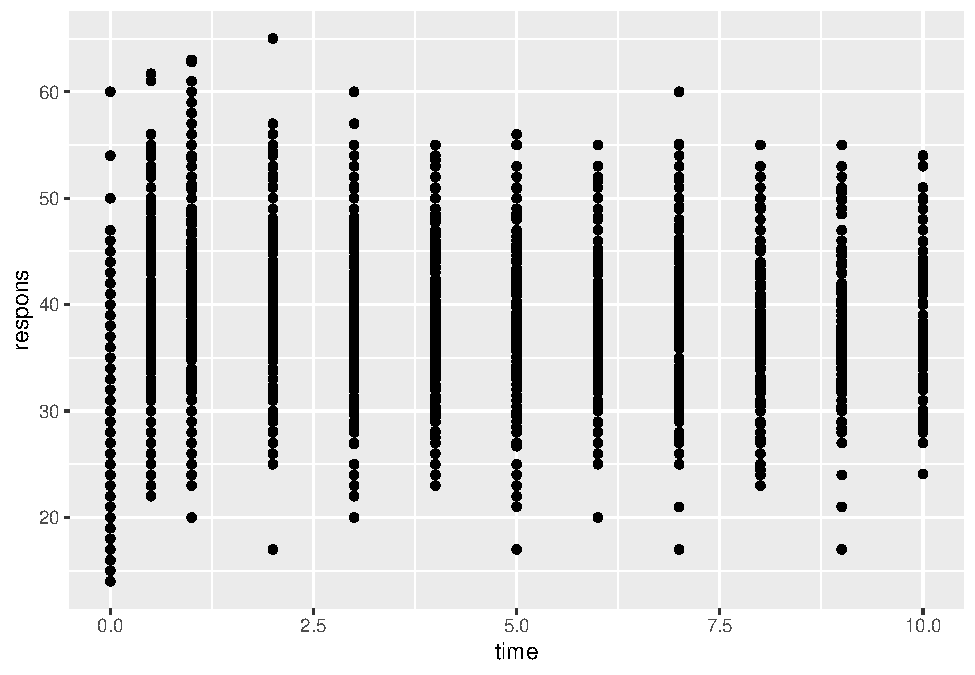
\includegraphics{LDA_Wan_files/figure-latex/unnamed-chunk-8-1.pdf}

\begin{Shaded}
\begin{Highlighting}[]
\CommentTok{\#Plot data with lm line}
\FunctionTok{ggplot}\NormalTok{(data, }\FunctionTok{aes}\NormalTok{(}\AttributeTok{x=}\NormalTok{time, }\AttributeTok{y=}\NormalTok{respons)) }\SpecialCharTok{+} \FunctionTok{geom\_point}\NormalTok{() }\SpecialCharTok{+} \FunctionTok{geom\_smooth}\NormalTok{(}\AttributeTok{method=}\StringTok{"lm"}\NormalTok{)}
\end{Highlighting}
\end{Shaded}

\begin{verbatim}
## `geom_smooth()` using formula = 'y ~ x'
\end{verbatim}

\begin{verbatim}
## Warning: Removed 4362 rows containing non-finite values (`stat_smooth()`).
## Removed 4362 rows containing missing values (`geom_point()`).
\end{verbatim}

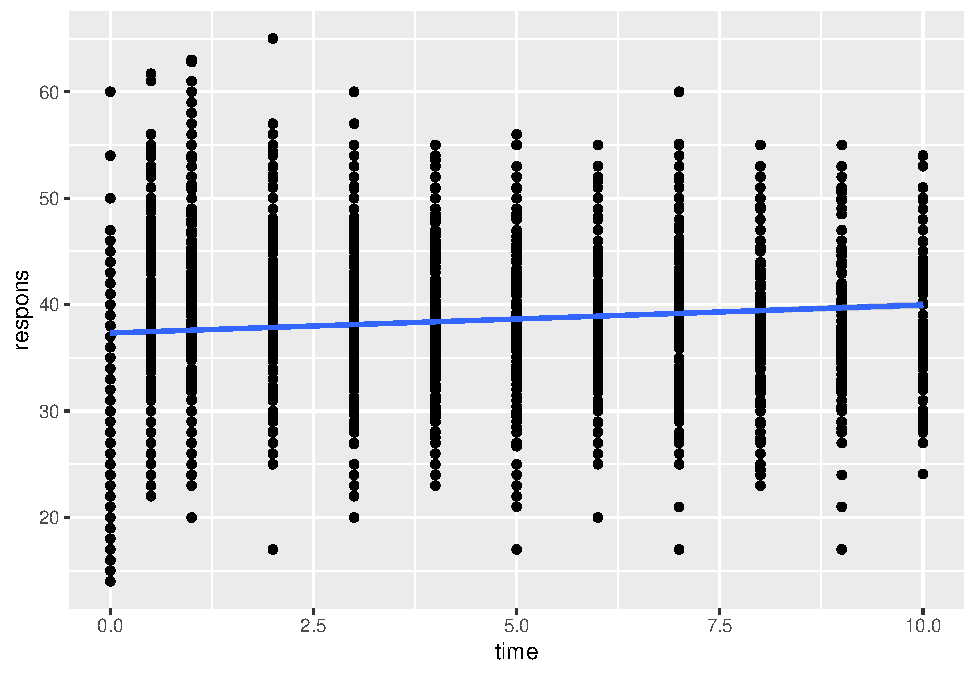
\includegraphics{LDA_Wan_files/figure-latex/unnamed-chunk-8-2.pdf}

\hypertarget{list-of-hypotheses-to-be-tested-by-the-data}{%
\subsection{1.3 List of Hypotheses to be tested by the
data}\label{list-of-hypotheses-to-be-tested-by-the-data}}

\begin{Shaded}
\begin{Highlighting}[]
\CommentTok{\#Select a sample of data to plot}
\FunctionTok{set.seed}\NormalTok{(}\DecValTok{1}\NormalTok{)}
\NormalTok{selected }\OtherTok{\textless{}{-}} \FunctionTok{sample}\NormalTok{(}\DecValTok{1}\SpecialCharTok{:}\FunctionTok{length}\NormalTok{(}\FunctionTok{unique}\NormalTok{(trenal.long}\SpecialCharTok{$}\NormalTok{id)),}\DecValTok{30}\NormalTok{,}\AttributeTok{replace=}\NormalTok{T) }\CommentTok{\# random samples and permutations}
\CommentTok{\#selected.vector = as.vector(selected)}
\NormalTok{data.selected }\OtherTok{=}\NormalTok{ data[(data}\SpecialCharTok{$}\NormalTok{id }\SpecialCharTok{\%in\%} \FunctionTok{c}\NormalTok{(selected)), ] }
\end{Highlighting}
\end{Shaded}

\begin{Shaded}
\begin{Highlighting}[]
\CommentTok{\# Individual plots}
\FunctionTok{plot}\NormalTok{(data.selected) }\CommentTok{\# WHAT I WILL GET FROM THE PLOT(DATA), HOW to plot a scatter plot of HC level changes with time for each id instead of a scatter plot}
\end{Highlighting}
\end{Shaded}

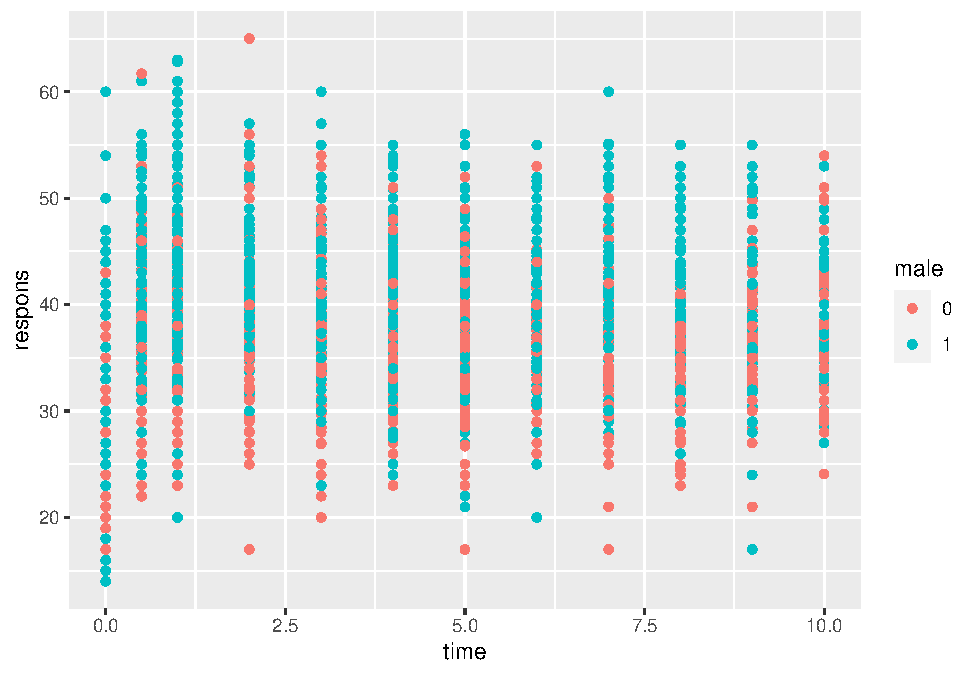
\includegraphics{LDA_Wan_files/figure-latex/unnamed-chunk-10-1.pdf}

\begin{Shaded}
\begin{Highlighting}[]
\CommentTok{\# spaghettic plot}
\FunctionTok{ggplot}\NormalTok{(data.selected,}\FunctionTok{aes}\NormalTok{(}\AttributeTok{x=}\NormalTok{time,}\AttributeTok{y=}\NormalTok{respons,}\AttributeTok{group=}\NormalTok{id,}\AttributeTok{color=}\NormalTok{id))}\SpecialCharTok{+}\FunctionTok{geom\_point}\NormalTok{()}\SpecialCharTok{+} \FunctionTok{geom\_line}\NormalTok{()}
\end{Highlighting}
\end{Shaded}

\begin{verbatim}
## Warning: Removed 106 rows containing missing values (`geom_point()`).
\end{verbatim}

\begin{verbatim}
## Warning: Removed 106 rows containing missing values (`geom_line()`).
\end{verbatim}

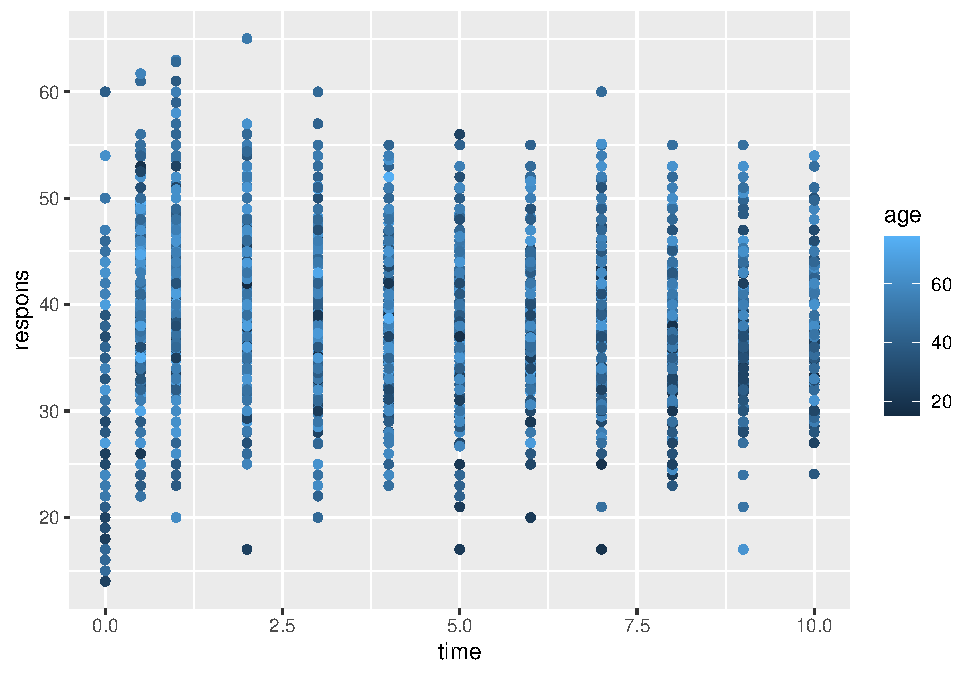
\includegraphics{LDA_Wan_files/figure-latex/unnamed-chunk-11-1.pdf}

\begin{Shaded}
\begin{Highlighting}[]
\CommentTok{\# Plot individual data by sex}
\FunctionTok{ggplot}\NormalTok{(data.selected,}\FunctionTok{aes}\NormalTok{(}\AttributeTok{x=}\NormalTok{time,}\AttributeTok{y=}\NormalTok{ respons,}\AttributeTok{group=}\NormalTok{id, }\AttributeTok{color=}\NormalTok{male))}\SpecialCharTok{+}\FunctionTok{geom\_point}\NormalTok{()}\SpecialCharTok{+}\FunctionTok{geom\_line}\NormalTok{()}
\end{Highlighting}
\end{Shaded}

\begin{verbatim}
## Warning: Removed 106 rows containing missing values (`geom_point()`).
\end{verbatim}

\begin{verbatim}
## Warning: Removed 106 rows containing missing values (`geom_line()`).
\end{verbatim}

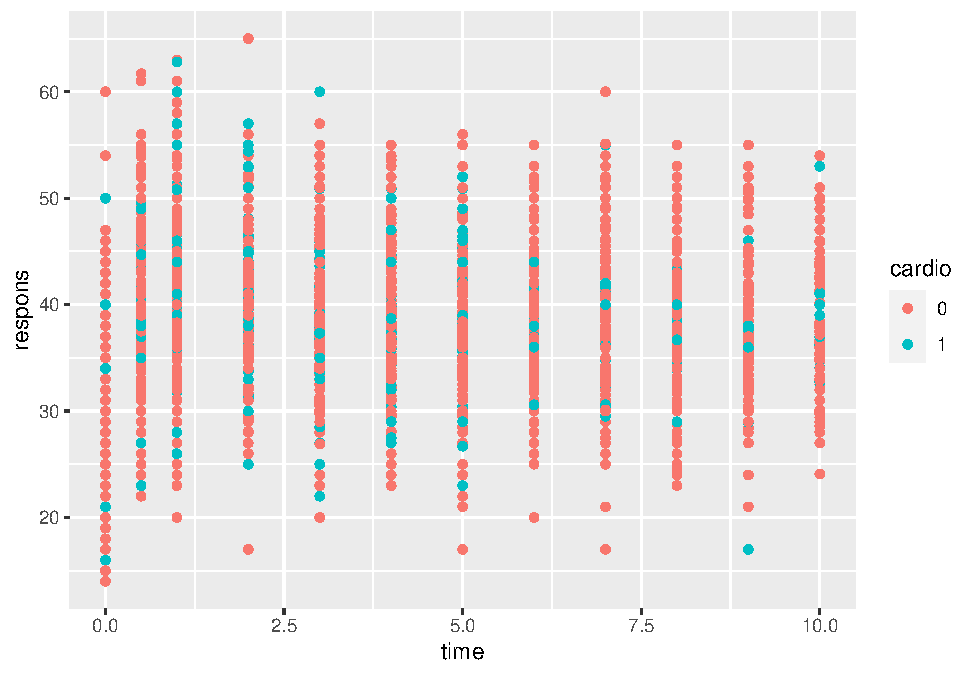
\includegraphics{LDA_Wan_files/figure-latex/unnamed-chunk-12-1.pdf}

\begin{Shaded}
\begin{Highlighting}[]
\CommentTok{\# Plot mean of male and mean of female}
\FunctionTok{library}\NormalTok{(dplyr)}
\NormalTok{MEAN }\OtherTok{\textless{}{-}}\NormalTok{ data.selected }\SpecialCharTok{\%\textgreater{}\%}
  \FunctionTok{group\_by}\NormalTok{(male,age,cardio,reject) }\SpecialCharTok{\%\textgreater{}\%}
  \FunctionTok{summarise}\NormalTok{(}\AttributeTok{respons =} \FunctionTok{mean}\NormalTok{(respons))}
\end{Highlighting}
\end{Shaded}

\begin{verbatim}
## `summarise()` has grouped output by 'male', 'age', 'cardio'. You can override
## using the `.groups` argument.
\end{verbatim}

\begin{Shaded}
\begin{Highlighting}[]
\NormalTok{MEAN}
\end{Highlighting}
\end{Shaded}

\begin{verbatim}
## # A tibble: 29 x 5
## # Groups:   male, age, cardio [28]
##     male   age cardio reject respons
##    <dbl> <dbl>  <dbl>  <dbl>   <dbl>
##  1     0    21      0      1    37.2
##  2     0    33      0      0    NA  
##  3     0    35      0      0    NA  
##  4     0    37      0      1    37.1
##  5     0    38      0      1    NA  
##  6     0    39      0      0    NA  
##  7     0    48      0      0    NA  
##  8     0    48      0      1    NA  
##  9     0    49      0      0    NA  
## 10     0    56      0      0    36.8
## # ... with 19 more rows
\end{verbatim}

\begin{Shaded}
\begin{Highlighting}[]
\FunctionTok{ggplot}\NormalTok{(data.selected,}\FunctionTok{aes}\NormalTok{(}\AttributeTok{x=}\NormalTok{age,}\AttributeTok{y=}\NormalTok{respons,}\AttributeTok{color=}\NormalTok{male)) }\SpecialCharTok{+} \FunctionTok{geom\_line}\NormalTok{(}\AttributeTok{data=}\NormalTok{MEAN)}
\end{Highlighting}
\end{Shaded}

\begin{verbatim}
## Warning: Removed 3 rows containing missing values (`geom_line()`).
\end{verbatim}

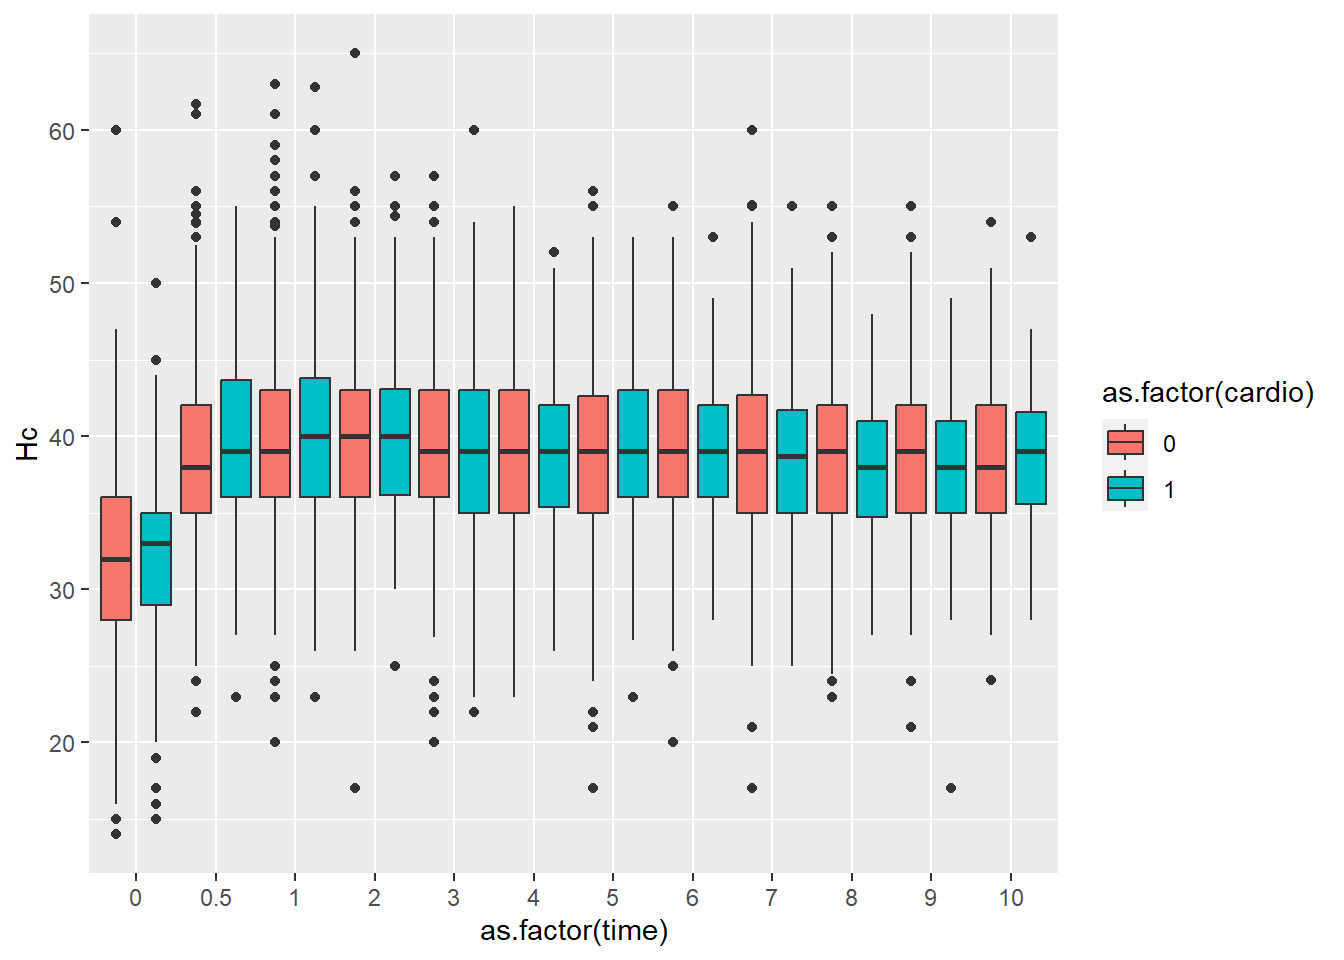
\includegraphics{LDA_Wan_files/figure-latex/unnamed-chunk-14-1.pdf}

\begin{Shaded}
\begin{Highlighting}[]
\CommentTok{\# Spaghetti Ggplot separated by male =1}
\NormalTok{p }\OtherTok{\textless{}{-}} \FunctionTok{ggplot}\NormalTok{(}\AttributeTok{data=}\NormalTok{data.selected,}\FunctionTok{aes}\NormalTok{(}\AttributeTok{x=}\NormalTok{time,}\AttributeTok{y=}\NormalTok{respons,}\AttributeTok{group=}\NormalTok{id))}
\NormalTok{p }\OtherTok{\textless{}{-}}\NormalTok{ p }\SpecialCharTok{+} \FunctionTok{geom\_line}\NormalTok{(}\AttributeTok{col=}\StringTok{"grey"}\NormalTok{)}\SpecialCharTok{+}\FunctionTok{stat\_summary}\NormalTok{(}\FunctionTok{aes}\NormalTok{(}\AttributeTok{group=}\DecValTok{1}\NormalTok{),}\AttributeTok{geom=}\StringTok{"line"}\NormalTok{,}\AttributeTok{fun=}\NormalTok{mean,}\AttributeTok{linewidth=}\DecValTok{2}\NormalTok{)}
\NormalTok{p }\SpecialCharTok{+} \FunctionTok{facet\_grid}\NormalTok{(}\SpecialCharTok{\textasciitilde{}}\NormalTok{male,}\AttributeTok{labeller=}\NormalTok{label\_both)}
\end{Highlighting}
\end{Shaded}

\begin{verbatim}
## Warning: Removed 106 rows containing non-finite values (`stat_summary()`).
\end{verbatim}

\begin{verbatim}
## Warning: Removed 106 rows containing missing values (`geom_line()`).
\end{verbatim}

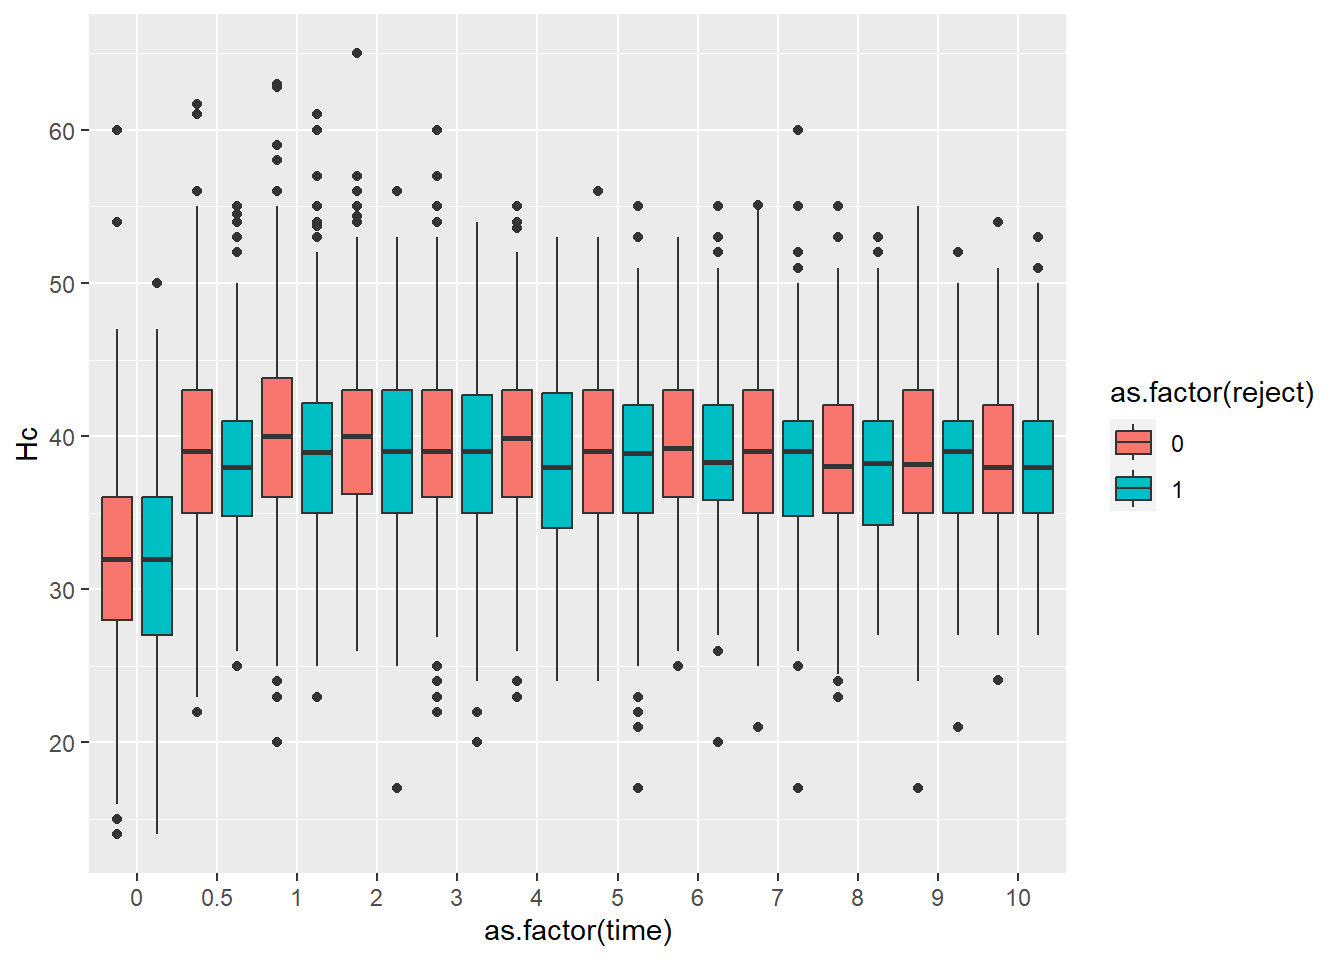
\includegraphics{LDA_Wan_files/figure-latex/unnamed-chunk-15-1.pdf}

\begin{Shaded}
\begin{Highlighting}[]
\CommentTok{\# Spaghetti Ggplot separated by cardio}
\NormalTok{p }\OtherTok{\textless{}{-}} \FunctionTok{ggplot}\NormalTok{(}\AttributeTok{data=}\NormalTok{data.selected,}\FunctionTok{aes}\NormalTok{(}\AttributeTok{x=}\NormalTok{time,}\AttributeTok{y=}\NormalTok{respons,}\AttributeTok{group=}\NormalTok{id))}
\NormalTok{p }\OtherTok{\textless{}{-}}\NormalTok{ p }\SpecialCharTok{+} \FunctionTok{geom\_line}\NormalTok{(}\AttributeTok{col=}\StringTok{"grey"}\NormalTok{)}\SpecialCharTok{+}\FunctionTok{stat\_summary}\NormalTok{(}\FunctionTok{aes}\NormalTok{(}\AttributeTok{group=}\DecValTok{1}\NormalTok{),}\AttributeTok{geom=}\StringTok{"line"}\NormalTok{,}\AttributeTok{fun=}\NormalTok{mean,}\AttributeTok{linewidth=}\DecValTok{2}\NormalTok{)}
\NormalTok{cardio.labs }\OtherTok{\textless{}{-}} \FunctionTok{c}\NormalTok{(}\StringTok{"Cardio = 0"}\NormalTok{,}\StringTok{"Cardio = 1"}\NormalTok{)}
\NormalTok{p }\SpecialCharTok{+} \FunctionTok{facet\_grid}\NormalTok{(}\SpecialCharTok{\textasciitilde{}}\NormalTok{cardio,}\AttributeTok{labeller =}\NormalTok{ label\_both) }
\end{Highlighting}
\end{Shaded}

\begin{verbatim}
## Warning: Removed 106 rows containing non-finite values (`stat_summary()`).
\end{verbatim}

\begin{verbatim}
## Warning: Removed 106 rows containing missing values (`geom_line()`).
\end{verbatim}

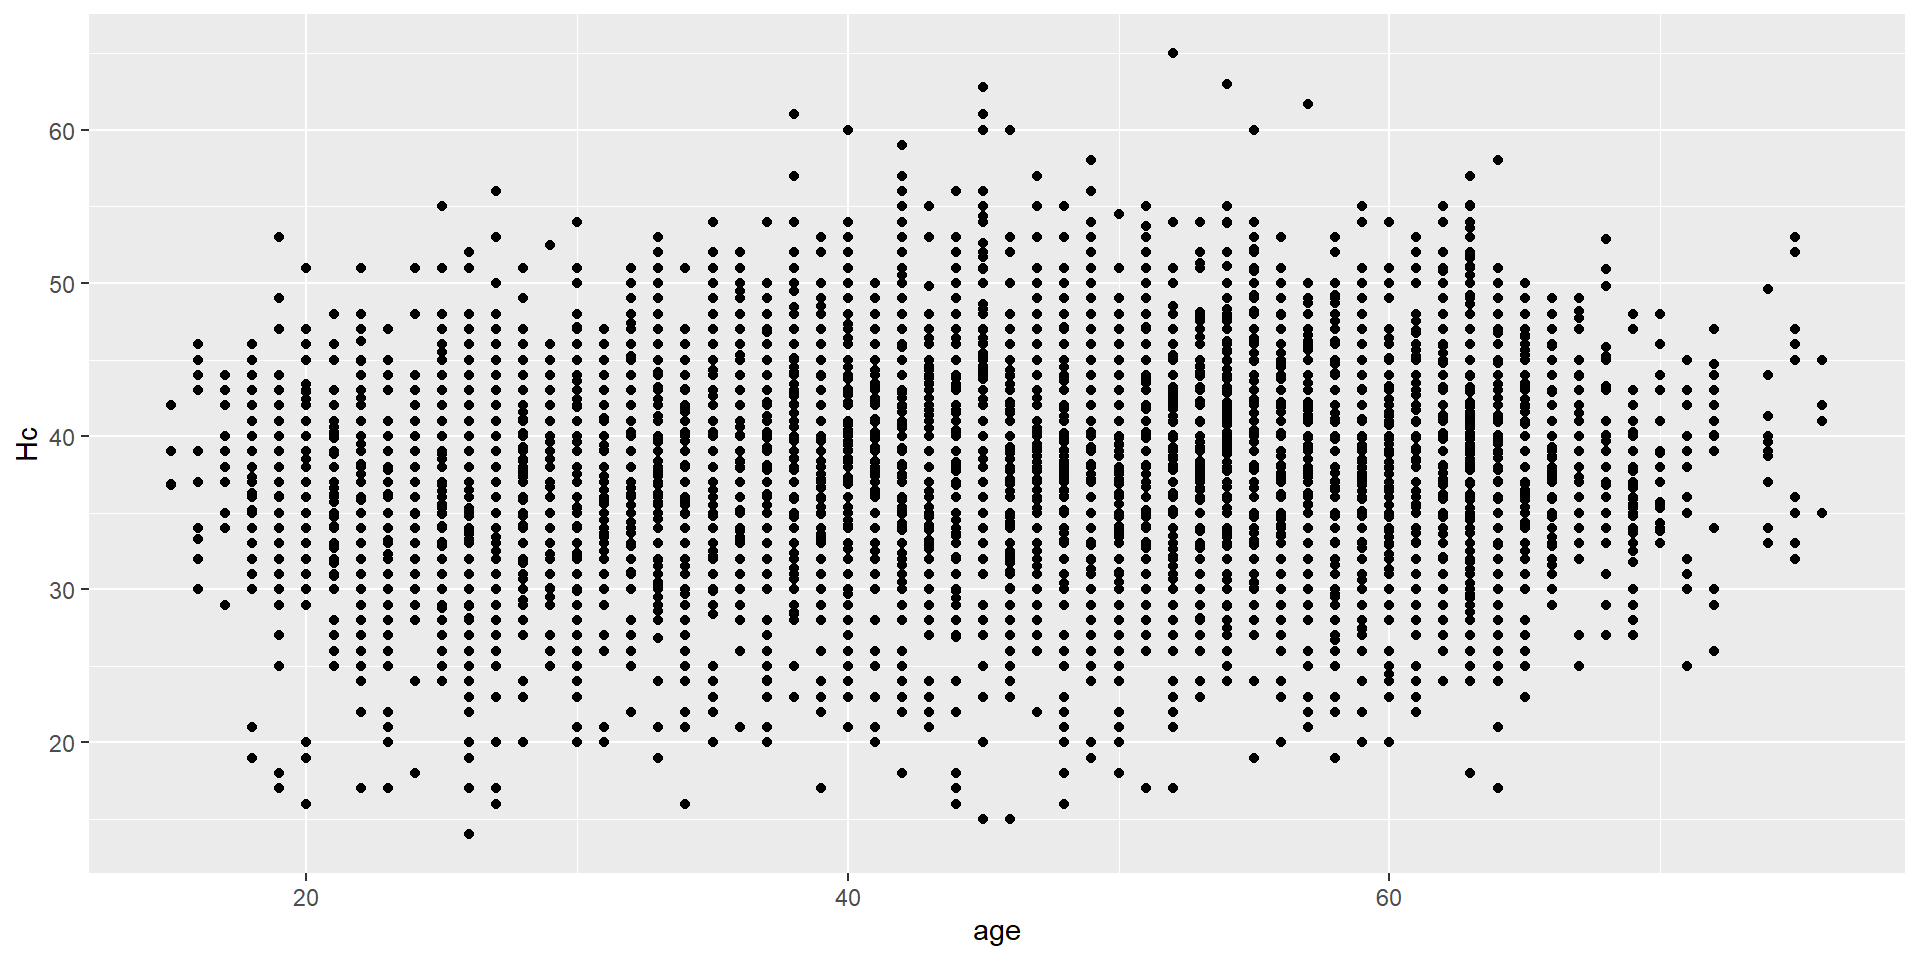
\includegraphics{LDA_Wan_files/figure-latex/unnamed-chunk-16-1.pdf}

\begin{Shaded}
\begin{Highlighting}[]
\CommentTok{\#p + facet\_grid(\textasciitilde{}cardio,labeller = labeller (cardio = cardio.labs)) }
\end{Highlighting}
\end{Shaded}

\begin{Shaded}
\begin{Highlighting}[]
\CommentTok{\# Spaghetti Ggplot separated by reject =1}
\NormalTok{p }\OtherTok{\textless{}{-}} \FunctionTok{ggplot}\NormalTok{(}\AttributeTok{data=}\NormalTok{data.selected,}\FunctionTok{aes}\NormalTok{(}\AttributeTok{x=}\NormalTok{time,}\AttributeTok{y=}\NormalTok{respons,}\AttributeTok{group=}\NormalTok{id))}
\NormalTok{p }\OtherTok{\textless{}{-}}\NormalTok{ p }\SpecialCharTok{+} \FunctionTok{geom\_line}\NormalTok{(}\AttributeTok{col=}\StringTok{"grey"}\NormalTok{)}\SpecialCharTok{+}\FunctionTok{stat\_summary}\NormalTok{(}\FunctionTok{aes}\NormalTok{(}\AttributeTok{group=}\DecValTok{1}\NormalTok{),}\AttributeTok{geom=}\StringTok{"line"}\NormalTok{,}\AttributeTok{fun=}\NormalTok{mean,}\AttributeTok{linewidth=}\DecValTok{2}\NormalTok{)}
\NormalTok{p }\SpecialCharTok{+} \FunctionTok{facet\_grid}\NormalTok{(}\SpecialCharTok{\textasciitilde{}}\NormalTok{reject,}\AttributeTok{labeller=}\NormalTok{label\_both)}
\end{Highlighting}
\end{Shaded}

\begin{verbatim}
## Warning: Removed 106 rows containing non-finite values (`stat_summary()`).
\end{verbatim}

\begin{verbatim}
## Warning: Removed 106 rows containing missing values (`geom_line()`).
\end{verbatim}

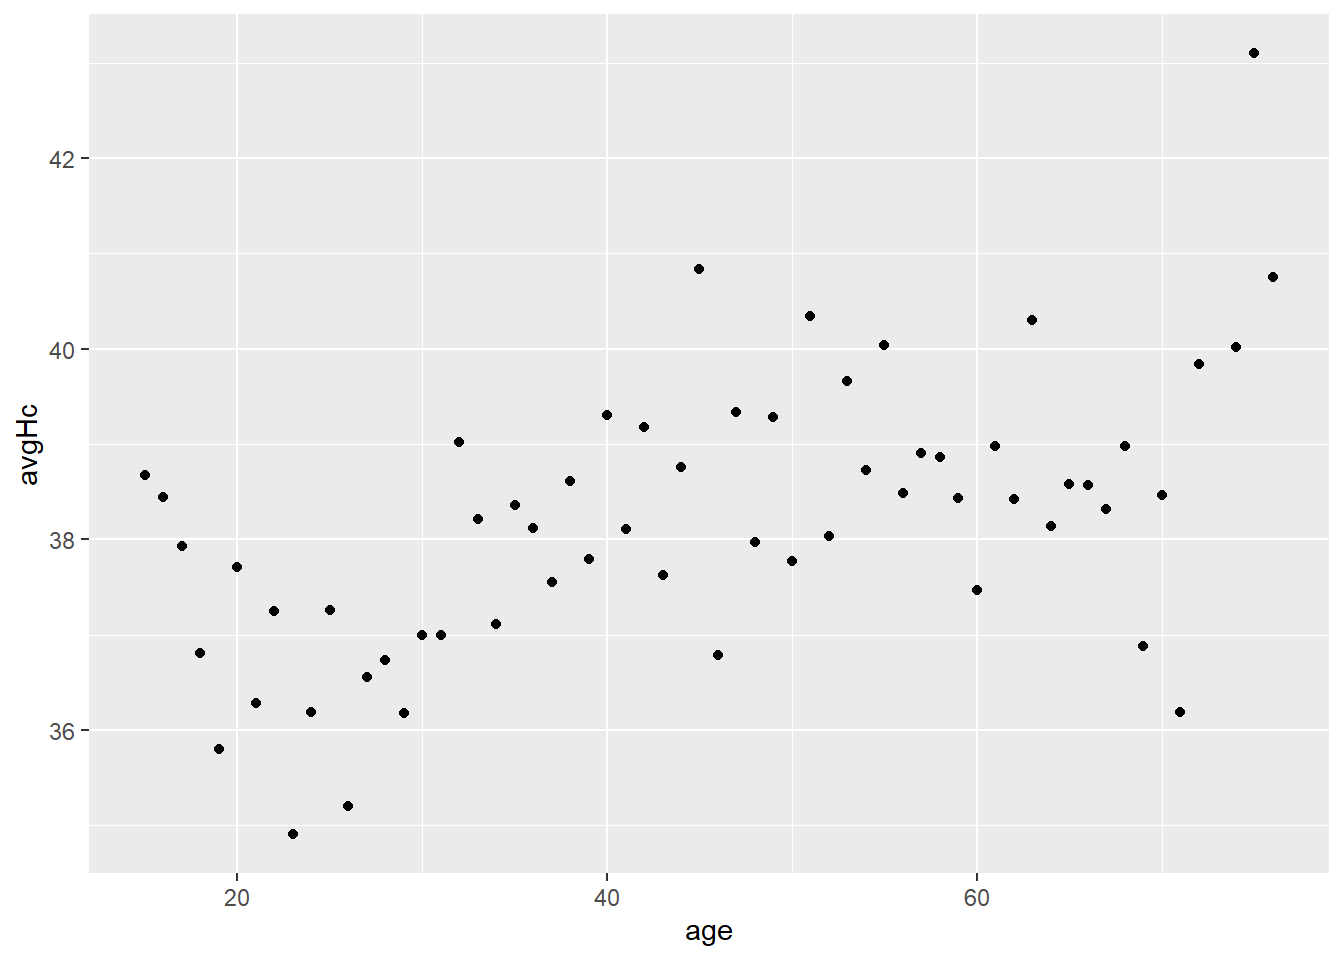
\includegraphics{LDA_Wan_files/figure-latex/unnamed-chunk-17-1.pdf}

\begin{Shaded}
\begin{Highlighting}[]
\CommentTok{\# BoxPlot}
\FunctionTok{ggplot}\NormalTok{(data.selected,}\FunctionTok{aes}\NormalTok{(}\AttributeTok{x=}\FunctionTok{as.factor}\NormalTok{(age),}\AttributeTok{y=}\NormalTok{respons))}\SpecialCharTok{+} \FunctionTok{geom\_boxplot}\NormalTok{(}\AttributeTok{position=}\FunctionTok{position\_dodge}\NormalTok{(}\DecValTok{1}\NormalTok{))}
\end{Highlighting}
\end{Shaded}

\begin{verbatim}
## Warning: Removed 106 rows containing non-finite values (`stat_boxplot()`).
\end{verbatim}

\includegraphics{LDA_Wan_files/figure-latex/unnamed-chunk-18-1.pdf}

\begin{Shaded}
\begin{Highlighting}[]
\CommentTok{\# BoxPlot}
\FunctionTok{ggplot}\NormalTok{(data.selected,}\FunctionTok{aes}\NormalTok{(}\AttributeTok{x=}\FunctionTok{as.factor}\NormalTok{(time),}\AttributeTok{y=}\NormalTok{respons))}\SpecialCharTok{+} \FunctionTok{geom\_boxplot}\NormalTok{(}\AttributeTok{position=}\FunctionTok{position\_dodge}\NormalTok{(}\DecValTok{1}\NormalTok{))}
\end{Highlighting}
\end{Shaded}

\begin{verbatim}
## Warning: Removed 106 rows containing non-finite values (`stat_boxplot()`).
\end{verbatim}

\includegraphics{LDA_Wan_files/figure-latex/unnamed-chunk-19-1.pdf}

\begin{Shaded}
\begin{Highlighting}[]
\CommentTok{\# Box plot by sex}
\FunctionTok{ggplot}\NormalTok{(data.selected,}\FunctionTok{aes}\NormalTok{(}\AttributeTok{x=}\FunctionTok{as.factor}\NormalTok{(time),}\AttributeTok{y=}\NormalTok{respons,}\AttributeTok{fill=}\FunctionTok{as.factor}\NormalTok{(male)))}\SpecialCharTok{+} 
  \FunctionTok{geom\_boxplot}\NormalTok{(}\AttributeTok{position=}\FunctionTok{position\_dodge}\NormalTok{(}\DecValTok{1}\NormalTok{))}
\end{Highlighting}
\end{Shaded}

\begin{verbatim}
## Warning: Removed 106 rows containing non-finite values (`stat_boxplot()`).
\end{verbatim}

\includegraphics{LDA_Wan_files/figure-latex/unnamed-chunk-20-1.pdf}

\begin{Shaded}
\begin{Highlighting}[]
\CommentTok{\# Box plot by cardio}
\FunctionTok{ggplot}\NormalTok{(data.selected,}\FunctionTok{aes}\NormalTok{(}\AttributeTok{x=}\FunctionTok{as.factor}\NormalTok{(time),}\AttributeTok{y=}\NormalTok{respons,}\AttributeTok{fill=}\FunctionTok{as.factor}\NormalTok{(cardio)))}\SpecialCharTok{+} 
  \FunctionTok{geom\_boxplot}\NormalTok{(}\AttributeTok{position=}\FunctionTok{position\_dodge}\NormalTok{(}\DecValTok{1}\NormalTok{))}
\end{Highlighting}
\end{Shaded}

\begin{verbatim}
## Warning: Removed 106 rows containing non-finite values (`stat_boxplot()`).
\end{verbatim}

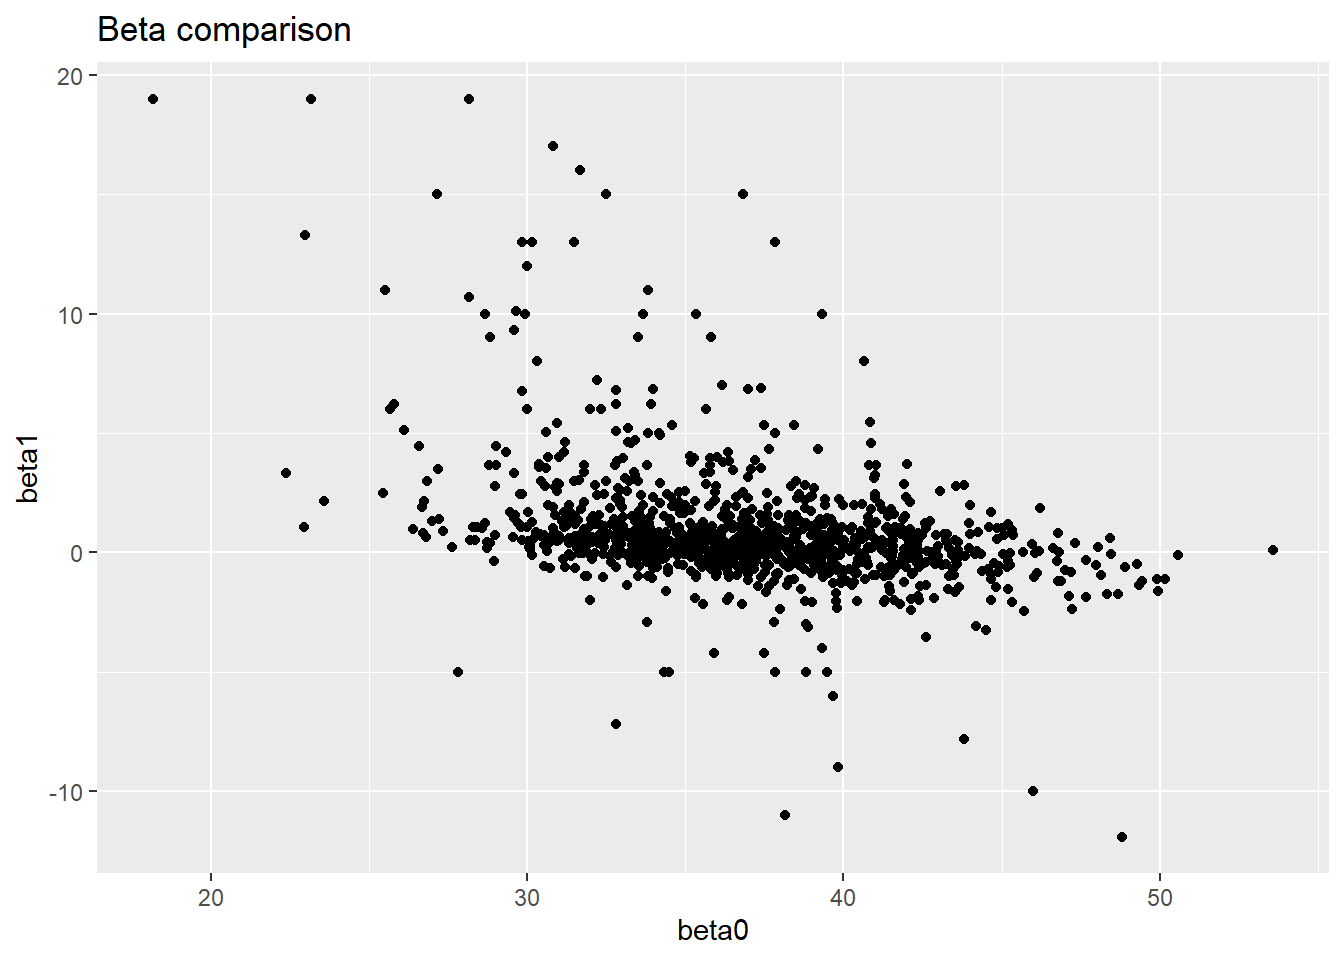
\includegraphics{LDA_Wan_files/figure-latex/unnamed-chunk-21-1.pdf}

\begin{Shaded}
\begin{Highlighting}[]
\CommentTok{\# Box plot by reject}
\FunctionTok{ggplot}\NormalTok{(data.selected,}\FunctionTok{aes}\NormalTok{(}\AttributeTok{x=}\FunctionTok{as.factor}\NormalTok{(time),}\AttributeTok{y=}\NormalTok{respons,}\AttributeTok{fill=}\FunctionTok{as.factor}\NormalTok{(reject)))}\SpecialCharTok{+} 
  \FunctionTok{geom\_boxplot}\NormalTok{(}\AttributeTok{position=}\FunctionTok{position\_dodge}\NormalTok{(}\DecValTok{1}\NormalTok{))}
\end{Highlighting}
\end{Shaded}

\begin{verbatim}
## Warning: Removed 106 rows containing non-finite values (`stat_boxplot()`).
\end{verbatim}

\includegraphics{LDA_Wan_files/figure-latex/unnamed-chunk-22-1.pdf}
\#\#\#\# Spaghetti Plot the response over time with the different
persons

\begin{Shaded}
\begin{Highlighting}[]
\CommentTok{\#data.selected = data[data$id == selected.vector,]\# why the dim(data.selected) = 12 x 8}
\CommentTok{\# Plot the respons over time for different id}
\CommentTok{\# If some responses are not available, NA}
\FunctionTok{ggplot}\NormalTok{(data.selected, }\FunctionTok{aes}\NormalTok{(}\AttributeTok{x=}\NormalTok{time, }\AttributeTok{y=}\NormalTok{respons, }\AttributeTok{group=}\NormalTok{id,}\AttributeTok{color=}\NormalTok{id)) }\SpecialCharTok{+} \FunctionTok{geom\_point}\NormalTok{()  }\SpecialCharTok{+}\FunctionTok{geom\_line}\NormalTok{()}
\end{Highlighting}
\end{Shaded}

\begin{verbatim}
## Warning: Removed 106 rows containing missing values (`geom_point()`).
\end{verbatim}

\begin{verbatim}
## Warning: Removed 106 rows containing missing values (`geom_line()`).
\end{verbatim}

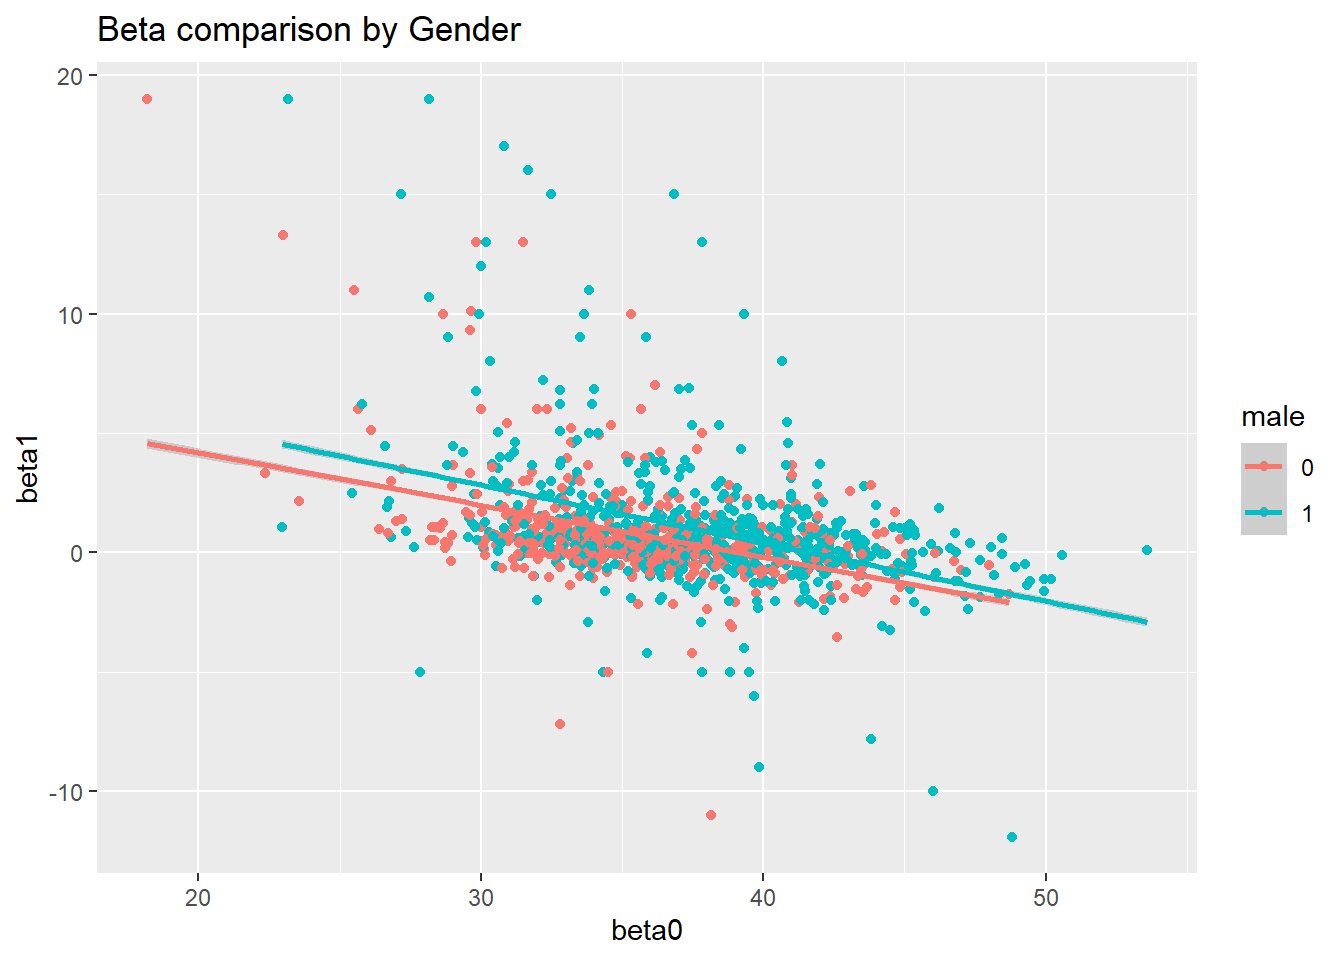
\includegraphics{LDA_Wan_files/figure-latex/unnamed-chunk-23-1.pdf}

\begin{Shaded}
\begin{Highlighting}[]
\CommentTok{\#ggplot(data.selected, aes(x=time, y=na.pass(respons), group=id,color=id)) + geom\_point()  +geom\_line()}
\end{Highlighting}
\end{Shaded}

\hypertarget{bax-plot-response-over-time}{%
\subparagraph{Bax plot response over
time}\label{bax-plot-response-over-time}}

\begin{Shaded}
\begin{Highlighting}[]
\CommentTok{\# Box plot}
\NormalTok{p }\OtherTok{\textless{}{-}} \FunctionTok{ggplot}\NormalTok{(data, }\FunctionTok{aes}\NormalTok{(}\AttributeTok{x=}\NormalTok{time, }\AttributeTok{y=}\NormalTok{respons,}\AttributeTok{group =}\NormalTok{time, }\AttributeTok{color =}\NormalTok{ time)) }\SpecialCharTok{+}  
  \FunctionTok{geom\_boxplot}\NormalTok{()}
\NormalTok{p}
\end{Highlighting}
\end{Shaded}

\begin{verbatim}
## Warning: Removed 4362 rows containing non-finite values (`stat_boxplot()`).
\end{verbatim}

\includegraphics{LDA_Wan_files/figure-latex/unnamed-chunk-24-1.pdf}
\#\#\#\# Hypothese one HC level will change with time differently if the
REJECT is different

\begin{Shaded}
\begin{Highlighting}[]
\CommentTok{\#Plot individual data}
\FunctionTok{ggplot}\NormalTok{(data, }\FunctionTok{aes}\NormalTok{(}\AttributeTok{x=}\NormalTok{time, }\AttributeTok{y=}\NormalTok{respons, }\AttributeTok{group=}\NormalTok{reject,}\AttributeTok{color=}\NormalTok{reject)) }\SpecialCharTok{+} \FunctionTok{geom\_point}\NormalTok{() }
\end{Highlighting}
\end{Shaded}

\begin{verbatim}
## Warning: Removed 4362 rows containing missing values (`geom_point()`).
\end{verbatim}

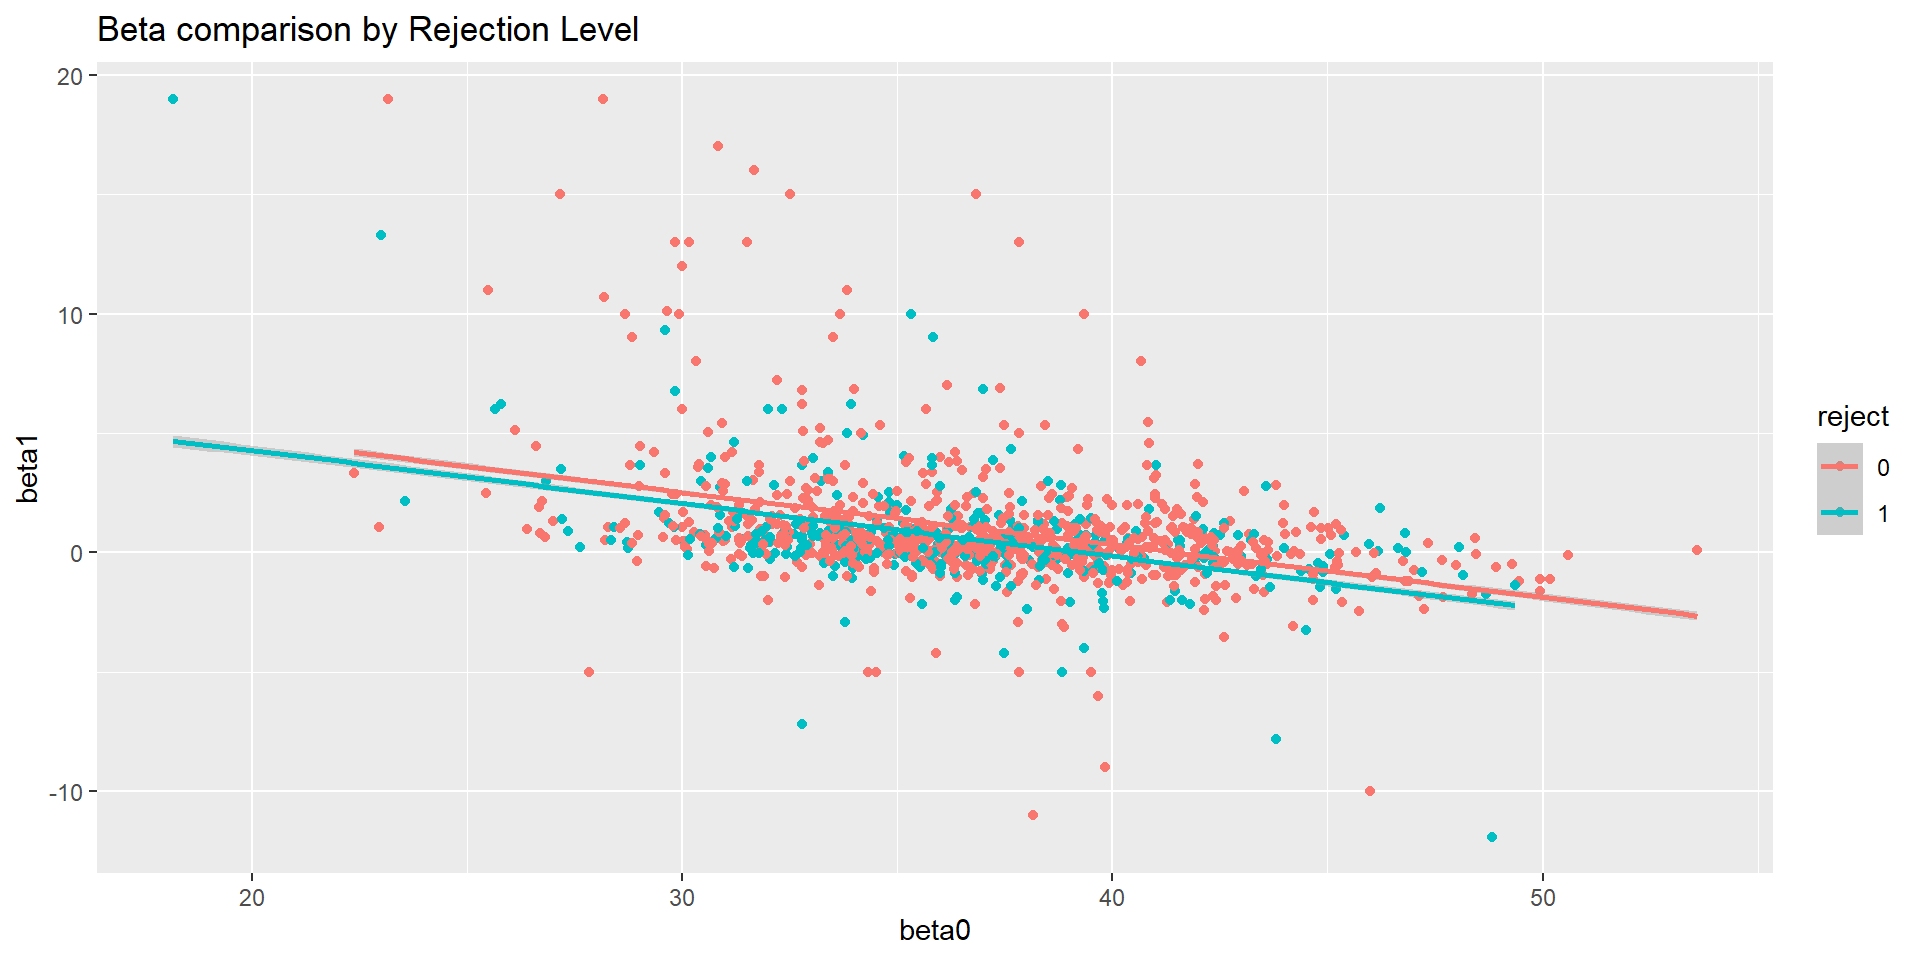
\includegraphics{LDA_Wan_files/figure-latex/unnamed-chunk-25-1.pdf}
\#\#\#\#\# Box plot

\begin{Shaded}
\begin{Highlighting}[]
\CommentTok{\# Box plot}
\NormalTok{p }\OtherTok{\textless{}{-}} \FunctionTok{ggplot}\NormalTok{(data, }\FunctionTok{aes}\NormalTok{(}\AttributeTok{x=}\NormalTok{reject, }\AttributeTok{y=}\NormalTok{respons,}\AttributeTok{group =}\NormalTok{ reject, }\AttributeTok{color =}\NormalTok{ reject)) }\SpecialCharTok{+}  
  \FunctionTok{geom\_boxplot}\NormalTok{()}
\NormalTok{p}
\end{Highlighting}
\end{Shaded}

\begin{verbatim}
## Warning: Removed 4362 rows containing non-finite values (`stat_boxplot()`).
\end{verbatim}

\includegraphics{LDA_Wan_files/figure-latex/unnamed-chunk-26-1.pdf}

\hypertarget{hypothese-two}{%
\paragraph{Hypothese two}\label{hypothese-two}}

HC level will change with time differently if the gender is different,
male (1) has generally higher HC level than female (0)

\begin{Shaded}
\begin{Highlighting}[]
\NormalTok{data.male }\OtherTok{=}\NormalTok{  data[(data}\SpecialCharTok{$}\NormalTok{male }\SpecialCharTok{==} \StringTok{"1"}\NormalTok{ ), ] }
\NormalTok{data.female }\OtherTok{=}\NormalTok{  data[(data}\SpecialCharTok{$}\NormalTok{male }\SpecialCharTok{==} \StringTok{"0"}\NormalTok{ ), ] }
\NormalTok{data.male.selected }\OtherTok{=}\NormalTok{  data[(data}\SpecialCharTok{$}\NormalTok{male }\SpecialCharTok{==} \StringTok{"1"} \SpecialCharTok{\&}\NormalTok{ data}\SpecialCharTok{$}\NormalTok{id }\SpecialCharTok{\%in\%} \FunctionTok{c}\NormalTok{(selected)), ] }
\NormalTok{data.female.selected }\OtherTok{=}\NormalTok{  data[(data}\SpecialCharTok{$}\NormalTok{male }\SpecialCharTok{==} \StringTok{"0"} \SpecialCharTok{\&}\NormalTok{ data}\SpecialCharTok{$}\NormalTok{id }\SpecialCharTok{\%in\%} \FunctionTok{c}\NormalTok{(selected)), ]}
\end{Highlighting}
\end{Shaded}

\hypertarget{spaghetti-plots-stratified-by-variables-gender-male}{%
\subparagraph{Spaghetti plots stratified by variables gender
male}\label{spaghetti-plots-stratified-by-variables-gender-male}}

\begin{Shaded}
\begin{Highlighting}[]
\FunctionTok{ggplot}\NormalTok{(data.male.selected, }\FunctionTok{aes}\NormalTok{(}\AttributeTok{x=}\NormalTok{time, }\AttributeTok{y =}\NormalTok{respons, }\AttributeTok{group=}\NormalTok{id,}\AttributeTok{color=}\NormalTok{id)) }\SpecialCharTok{+} \FunctionTok{geom\_point}\NormalTok{()  }\SpecialCharTok{+}\FunctionTok{geom\_line}\NormalTok{()}\SpecialCharTok{+}\FunctionTok{ggtitle}\NormalTok{(}\StringTok{"Spaghetti plot for male"}\NormalTok{)}\SpecialCharTok{+} \FunctionTok{geom\_smooth}\NormalTok{(}\AttributeTok{method=}\StringTok{"lm"}\NormalTok{)}
\end{Highlighting}
\end{Shaded}

\begin{verbatim}
## `geom_smooth()` using formula = 'y ~ x'
\end{verbatim}

\begin{verbatim}
## Warning: Removed 47 rows containing non-finite values (`stat_smooth()`).
\end{verbatim}

\begin{verbatim}
## Warning: Removed 47 rows containing missing values (`geom_point()`).
\end{verbatim}

\begin{verbatim}
## Warning: Removed 47 rows containing missing values (`geom_line()`).
\end{verbatim}

\includegraphics{LDA_Wan_files/figure-latex/unnamed-chunk-28-1.pdf}

\begin{Shaded}
\begin{Highlighting}[]
\FunctionTok{ggplot}\NormalTok{(data.female.selected, }\FunctionTok{aes}\NormalTok{(}\AttributeTok{x=}\NormalTok{time, }\AttributeTok{y=}\NormalTok{ respons, }\AttributeTok{group=}\NormalTok{id,}\AttributeTok{color=}\NormalTok{id)) }\SpecialCharTok{+} \FunctionTok{geom\_point}\NormalTok{()  }\SpecialCharTok{+}\FunctionTok{geom\_line}\NormalTok{()}\SpecialCharTok{+}\FunctionTok{ggtitle}\NormalTok{(}\StringTok{"Spaghetti plot for female"}\NormalTok{)}\SpecialCharTok{+} \FunctionTok{geom\_smooth}\NormalTok{(}\AttributeTok{method=}\StringTok{"lm"}\NormalTok{)}
\end{Highlighting}
\end{Shaded}

\begin{verbatim}
## `geom_smooth()` using formula = 'y ~ x'
\end{verbatim}

\begin{verbatim}
## Warning: Removed 59 rows containing non-finite values (`stat_smooth()`).
\end{verbatim}

\begin{verbatim}
## Warning: Removed 59 rows containing missing values (`geom_point()`).
\end{verbatim}

\begin{verbatim}
## Warning: Removed 59 rows containing missing values (`geom_line()`).
\end{verbatim}

\includegraphics{LDA_Wan_files/figure-latex/unnamed-chunk-28-2.pdf}
\#\#\#\#\# Box plot

\begin{Shaded}
\begin{Highlighting}[]
\NormalTok{p }\OtherTok{\textless{}{-}} \FunctionTok{ggplot}\NormalTok{(data, }\FunctionTok{aes}\NormalTok{(}\AttributeTok{x=}\NormalTok{time, }\AttributeTok{y=}\NormalTok{respons,}\AttributeTok{fill=}\NormalTok{ male)) }\SpecialCharTok{+}  
  \FunctionTok{geom\_boxplot}\NormalTok{()}
\NormalTok{p}
\end{Highlighting}
\end{Shaded}

\begin{verbatim}
## Warning: Continuous x aesthetic
## i did you forget `aes(group = ...)`?
\end{verbatim}

\begin{verbatim}
## Warning: Removed 4362 rows containing non-finite values (`stat_boxplot()`).
\end{verbatim}

\begin{verbatim}
## Warning: The following aesthetics were dropped during statistical transformation: fill
## i This can happen when ggplot fails to infer the correct grouping structure in
##   the data.
## i Did you forget to specify a `group` aesthetic or to convert a numerical
##   variable into a factor?
\end{verbatim}

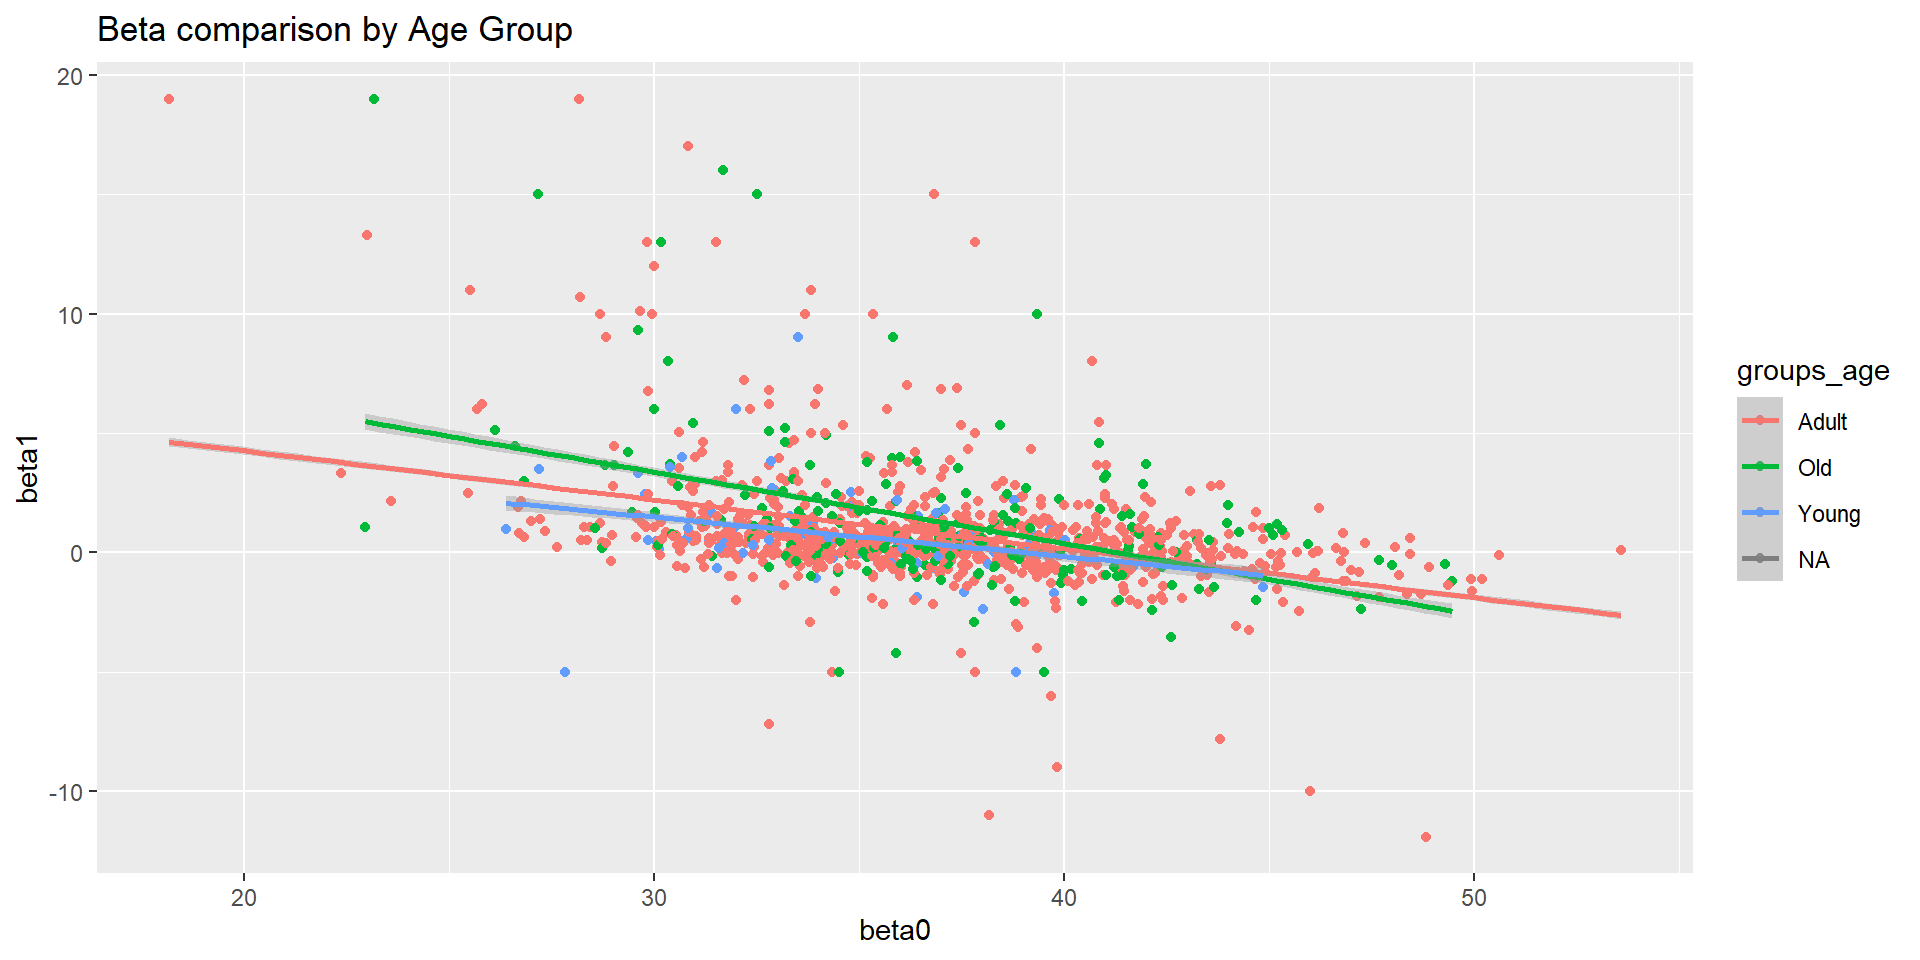
\includegraphics{LDA_Wan_files/figure-latex/unnamed-chunk-29-1.pdf}

\hypertarget{box-plot-for-male-and-female}{%
\subparagraph{Box plot for male and
female}\label{box-plot-for-male-and-female}}

COULD I PLOT THEM IN THE SAME FIGURE?

\begin{Shaded}
\begin{Highlighting}[]
\NormalTok{p.box.male }\OtherTok{\textless{}{-}} \FunctionTok{ggplot}\NormalTok{(data.male, }\FunctionTok{aes}\NormalTok{(}\AttributeTok{x=}\NormalTok{time, }\AttributeTok{y=}\NormalTok{respons,}\AttributeTok{group =}\NormalTok{ time, }\AttributeTok{color =}\NormalTok{ time)) }\SpecialCharTok{+}  
  \FunctionTok{geom\_boxplot}\NormalTok{()}
\NormalTok{p.box.male}
\end{Highlighting}
\end{Shaded}

\begin{verbatim}
## Warning: Removed 2647 rows containing non-finite values (`stat_boxplot()`).
\end{verbatim}

\includegraphics{LDA_Wan_files/figure-latex/unnamed-chunk-30-1.pdf}

\begin{Shaded}
\begin{Highlighting}[]
\NormalTok{p.box.female }\OtherTok{\textless{}{-}} \FunctionTok{ggplot}\NormalTok{(data.female, }\FunctionTok{aes}\NormalTok{(}\AttributeTok{x=}\NormalTok{time, }\AttributeTok{y=}\NormalTok{respons,}\AttributeTok{group =}\NormalTok{ time, }\AttributeTok{color =}\NormalTok{ time)) }\SpecialCharTok{+}  
  \FunctionTok{geom\_boxplot}\NormalTok{()}
\NormalTok{p.box.female}
\end{Highlighting}
\end{Shaded}

\begin{verbatim}
## Warning: Removed 1715 rows containing non-finite values (`stat_boxplot()`).
\end{verbatim}

\includegraphics{LDA_Wan_files/figure-latex/unnamed-chunk-30-2.pdf}

\hypertarget{hypothese-three}{%
\paragraph{Hypothese three}\label{hypothese-three}}

HC level will change with time differently if the age when performing
the kidney transplant is younger

\begin{Shaded}
\begin{Highlighting}[]
\CommentTok{\#Plot individual data}
\FunctionTok{ggplot}\NormalTok{(data.selected, }\FunctionTok{aes}\NormalTok{(}\AttributeTok{x=}\NormalTok{time, }\AttributeTok{y=}\NormalTok{respons, }\AttributeTok{group=}\NormalTok{age,}\AttributeTok{color=}\NormalTok{age)) }\SpecialCharTok{+} \FunctionTok{geom\_point}\NormalTok{() }\SpecialCharTok{+}\FunctionTok{geom\_line}\NormalTok{()}
\end{Highlighting}
\end{Shaded}

\begin{verbatim}
## Warning: Removed 106 rows containing missing values (`geom_point()`).
\end{verbatim}

\begin{verbatim}
## Warning: Removed 82 rows containing missing values (`geom_line()`).
\end{verbatim}

\includegraphics{LDA_Wan_files/figure-latex/unnamed-chunk-31-1.pdf}

\hypertarget{box-plot}{%
\subparagraph{Box plot}\label{box-plot}}

\begin{Shaded}
\begin{Highlighting}[]
\NormalTok{p }\OtherTok{\textless{}{-}} \FunctionTok{ggplot}\NormalTok{(data, }\FunctionTok{aes}\NormalTok{(}\AttributeTok{x=}\NormalTok{age, }\AttributeTok{y=}\NormalTok{respons,}\AttributeTok{group =}\NormalTok{ age, }\AttributeTok{color =}\NormalTok{ age)) }\SpecialCharTok{+}  
  \FunctionTok{geom\_boxplot}\NormalTok{()}
\NormalTok{p}
\end{Highlighting}
\end{Shaded}

\begin{verbatim}
## Warning: Removed 12 rows containing missing values (`stat_boxplot()`).
\end{verbatim}

\begin{verbatim}
## Warning: Removed 4357 rows containing non-finite values (`stat_boxplot()`).
\end{verbatim}

\includegraphics{LDA_Wan_files/figure-latex/unnamed-chunk-32-1.pdf}
\#\#\#\# Hypothese four HC level will change with time differently if
the patient has experienced cardio-vascular problem during the years
preceding the tranplantation \#\#\#\#\# Spathetti plot ?

\begin{Shaded}
\begin{Highlighting}[]
\CommentTok{\#Plot individual data}
\FunctionTok{ggplot}\NormalTok{(data.selected, }\FunctionTok{aes}\NormalTok{(}\AttributeTok{x=}\NormalTok{time, }\AttributeTok{y=}\NormalTok{respons, }\AttributeTok{group=}\NormalTok{cardio,}\AttributeTok{color=}\NormalTok{cardio)) }\SpecialCharTok{+} \FunctionTok{geom\_point}\NormalTok{()  }\SpecialCharTok{+}\FunctionTok{geom\_line}\NormalTok{()}
\end{Highlighting}
\end{Shaded}

\begin{verbatim}
## Warning: Removed 106 rows containing missing values (`geom_point()`).
\end{verbatim}

\begin{verbatim}
## Warning: Removed 30 rows containing missing values (`geom_line()`).
\end{verbatim}

\includegraphics{LDA_Wan_files/figure-latex/unnamed-chunk-33-1.pdf}
\#\#\#\#\# Bar plot

\begin{Shaded}
\begin{Highlighting}[]
\NormalTok{p }\OtherTok{\textless{}{-}} \FunctionTok{ggplot}\NormalTok{(data, }\FunctionTok{aes}\NormalTok{(}\AttributeTok{x=}\NormalTok{cardio, }\AttributeTok{y=}\NormalTok{respons,}\AttributeTok{group =}\NormalTok{ cardio, }\AttributeTok{color =}\NormalTok{ cardio)) }\SpecialCharTok{+}  
  \FunctionTok{geom\_boxplot}\NormalTok{()}
\NormalTok{p}
\end{Highlighting}
\end{Shaded}

\begin{verbatim}
## Warning: Removed 4362 rows containing non-finite values (`stat_boxplot()`).
\end{verbatim}

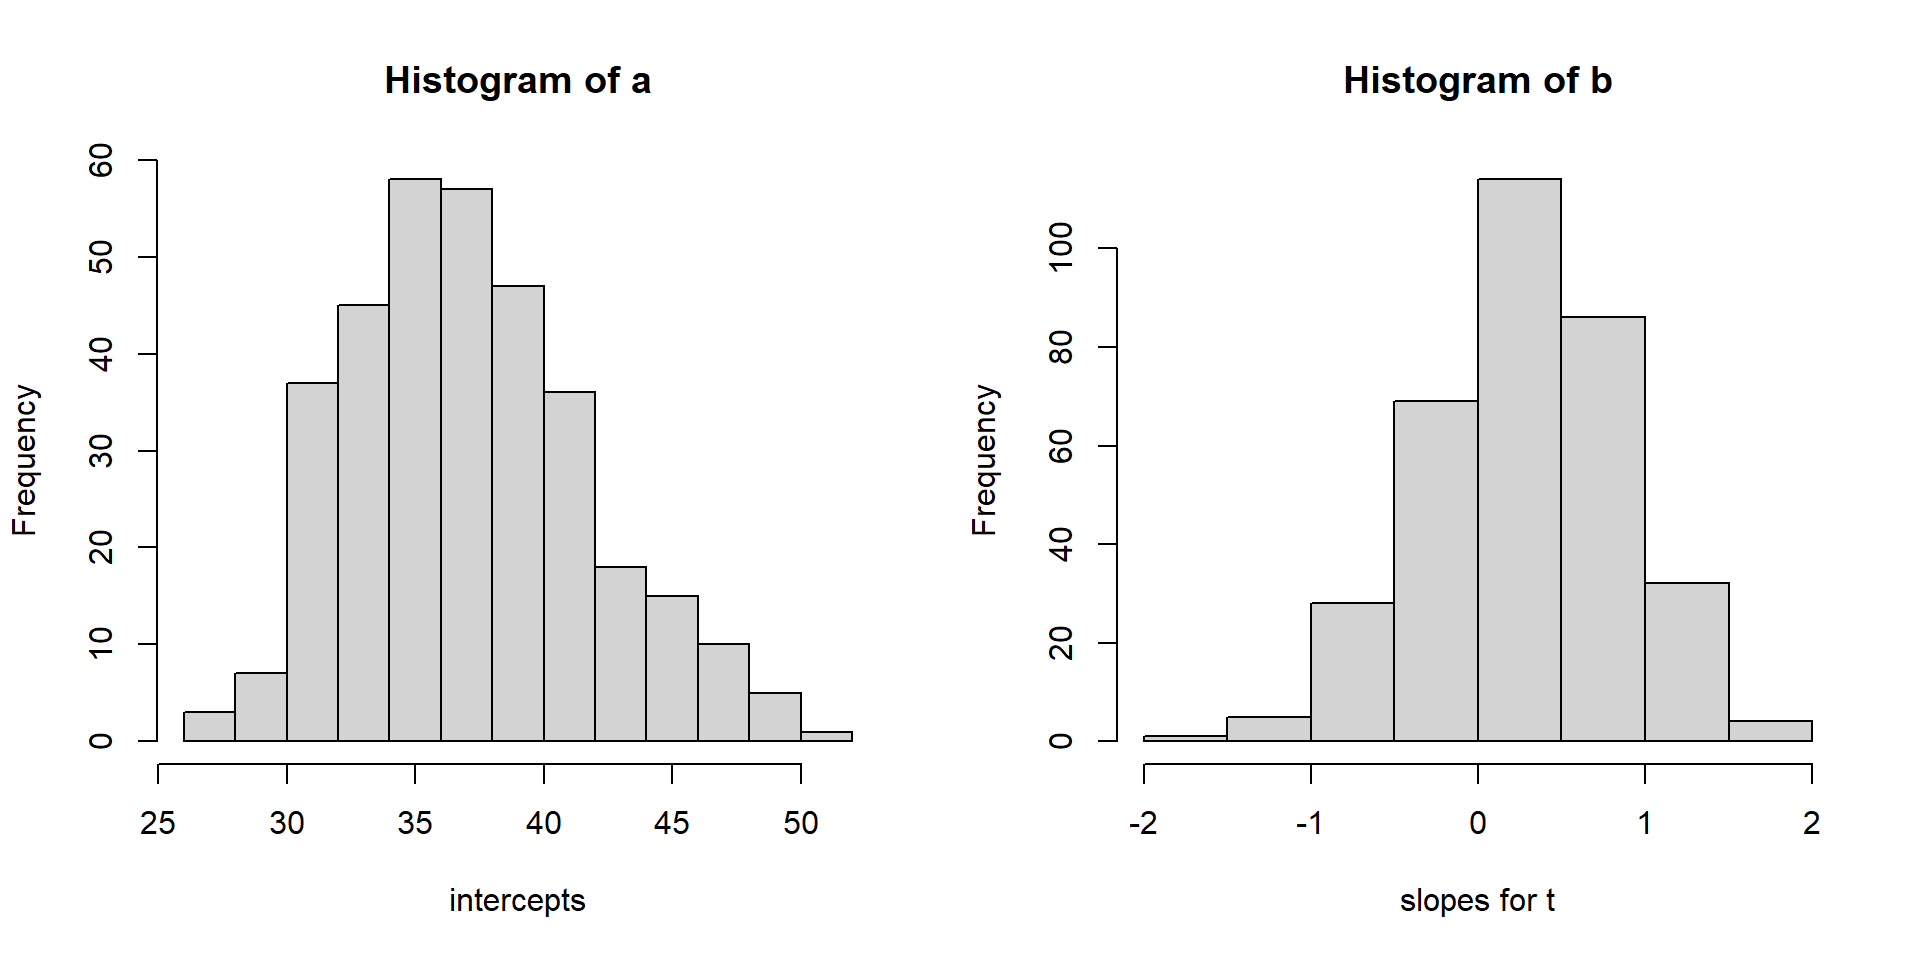
\includegraphics{LDA_Wan_files/figure-latex/unnamed-chunk-34-1.pdf}

\hypertarget{correlation-analysis-for-different-hc-levels-along-time}{%
\subsection{Correlation analysis for different HC levels along
time}\label{correlation-analysis-for-different-hc-levels-along-time}}

For this purpose we need the wide table

\begin{Shaded}
\begin{Highlighting}[]
\NormalTok{trenal.wide }\OtherTok{=}\NormalTok{ trenal[,}\DecValTok{1}\SpecialCharTok{:}\DecValTok{17}\NormalTok{]}
\FunctionTok{summary}\NormalTok{(trenal.wide)}
\end{Highlighting}
\end{Shaded}

\begin{verbatim}
##       HC0             HC06            HC1             HC2            HC3       
##  Min.   :14.00   Min.   :22.00   Min.   :20.00   Min.   :17.0   Min.   :20.00  
##  1st Qu.:28.00   1st Qu.:35.00   1st Qu.:36.00   1st Qu.:36.0   1st Qu.:36.00  
##  Median :32.00   Median :38.55   Median :39.00   Median :40.0   Median :39.00  
##  Mean   :31.86   Mean   :38.83   Mean   :39.71   Mean   :39.7   Mean   :39.17  
##  3rd Qu.:36.00   3rd Qu.:42.00   3rd Qu.:43.00   3rd Qu.:43.0   3rd Qu.:43.00  
##  Max.   :60.00   Max.   :61.70   Max.   :63.00   Max.   :65.0   Max.   :60.00  
##  NA's   :12                      NA's   :12      NA's   :1044   NA's   :2460   
##       HC4             HC5             HC6             HC7       
##  Min.   :23.00   Min.   :17.00   Min.   :20.00   Min.   :17.00  
##  1st Qu.:35.00   1st Qu.:35.00   1st Qu.:36.00   1st Qu.:35.00  
##  Median :39.00   Median :39.00   Median :39.00   Median :39.00  
##  Mean   :39.16   Mean   :39.02   Mean   :39.11   Mean   :38.85  
##  3rd Qu.:43.00   3rd Qu.:43.00   3rd Qu.:43.00   3rd Qu.:42.00  
##  Max.   :55.00   Max.   :56.00   Max.   :55.00   Max.   :60.00  
##  NA's   :3768    NA's   :5016    NA's   :6096    NA's   :7140   
##       HC8             HC9             HC10             id        
##  Min.   :23.00   Min.   :17.00   Min.   :24.10   Min.   :   1.0  
##  1st Qu.:35.00   1st Qu.:35.00   1st Qu.:35.00   1st Qu.: 290.8  
##  Median :38.05   Median :38.50   Median :38.00   Median : 580.5  
##  Mean   :38.35   Mean   :38.57   Mean   :38.49   Mean   : 580.5  
##  3rd Qu.:42.00   3rd Qu.:42.00   3rd Qu.:42.00   3rd Qu.: 870.2  
##  Max.   :55.00   Max.   :55.00   Max.   :54.00   Max.   :1160.0  
##  NA's   :8064    NA's   :8988    NA's   :9744                    
##       age             male            cardio           reject      
##  Min.   :15.00   Min.   :0.0000   Min.   :0.0000   Min.   :0.0000  
##  1st Qu.:36.00   1st Qu.:0.0000   1st Qu.:0.0000   1st Qu.:0.0000  
##  Median :48.00   Median :1.0000   Median :0.0000   Median :0.0000  
##  Mean   :46.43   Mean   :0.5741   Mean   :0.1784   Mean   :0.3164  
##  3rd Qu.:57.00   3rd Qu.:1.0000   3rd Qu.:0.0000   3rd Qu.:1.0000  
##  Max.   :76.00   Max.   :1.0000   Max.   :1.0000   Max.   :1.0000  
##  NA's   :12
\end{verbatim}

\begin{Shaded}
\begin{Highlighting}[]
\FunctionTok{cor}\NormalTok{(trenal.wide}\SpecialCharTok{$}\NormalTok{HC0,trenal.wide}\SpecialCharTok{$}\NormalTok{HC06)}
\end{Highlighting}
\end{Shaded}

\begin{verbatim}
## [1] NA
\end{verbatim}

\begin{Shaded}
\begin{Highlighting}[]
\CommentTok{\# scatter plot matrix}

\FunctionTok{pairs}\NormalTok{(}\SpecialCharTok{\textasciitilde{}}\NormalTok{HC0}\SpecialCharTok{+}\NormalTok{HC06}\SpecialCharTok{+}\NormalTok{HC1}\SpecialCharTok{+}\NormalTok{HC2}\SpecialCharTok{+}\NormalTok{HC3}\SpecialCharTok{+}\NormalTok{HC4}\SpecialCharTok{+}\NormalTok{HC5}\SpecialCharTok{+}\NormalTok{HC6}\SpecialCharTok{+}\NormalTok{HC7}\SpecialCharTok{+}\NormalTok{HC8}\SpecialCharTok{+}\NormalTok{HC9}\SpecialCharTok{+}\NormalTok{HC10,}\AttributeTok{data=}\NormalTok{trenal.wide,}
   \AttributeTok{main=}\StringTok{"Simple Scatterplot Matrix"}\NormalTok{)}
\end{Highlighting}
\end{Shaded}

\includegraphics{LDA_Wan_files/figure-latex/unnamed-chunk-38-1.pdf}

\begin{Shaded}
\begin{Highlighting}[]
\CommentTok{\#Plot individual data}
\FunctionTok{ggplot}\NormalTok{(data, }\FunctionTok{aes}\NormalTok{(}\AttributeTok{x=}\NormalTok{time, }\AttributeTok{y=}\NormalTok{respons, }\AttributeTok{group=}\NormalTok{male,}\AttributeTok{color=}\NormalTok{male)) }\SpecialCharTok{+} \FunctionTok{geom\_point}\NormalTok{() }
\end{Highlighting}
\end{Shaded}

\begin{verbatim}
## Warning: Removed 4362 rows containing missing values (`geom_point()`).
\end{verbatim}

\includegraphics{LDA_Wan_files/figure-latex/unnamed-chunk-39-1.pdf}

\begin{Shaded}
\begin{Highlighting}[]
\CommentTok{\#Spaghetti Plot}
\FunctionTok{ggplot}\NormalTok{(data, }\FunctionTok{aes}\NormalTok{(}\AttributeTok{x=}\NormalTok{time, }\AttributeTok{y=}\NormalTok{respons, }\AttributeTok{group=}\NormalTok{male,}\AttributeTok{color=}\NormalTok{male)) }\SpecialCharTok{+} \FunctionTok{geom\_point}\NormalTok{() }\SpecialCharTok{+}\FunctionTok{geom\_line}\NormalTok{()}
\end{Highlighting}
\end{Shaded}

\begin{verbatim}
## Warning: Removed 4362 rows containing missing values (`geom_point()`).
\end{verbatim}

\begin{verbatim}
## Warning: Removed 638 rows containing missing values (`geom_line()`).
\end{verbatim}

\includegraphics{LDA_Wan_files/figure-latex/unnamed-chunk-39-2.pdf}

\begin{Shaded}
\begin{Highlighting}[]
\CommentTok{\#Spaghetti with fitted lines}
\FunctionTok{ggplot}\NormalTok{(data, }\FunctionTok{aes}\NormalTok{(}\AttributeTok{x=}\NormalTok{time, }\AttributeTok{y=}\NormalTok{respons, }\AttributeTok{group=}\NormalTok{male,}\AttributeTok{color=}\NormalTok{male)) }\SpecialCharTok{+} \FunctionTok{geom\_point}\NormalTok{()}\SpecialCharTok{+} \FunctionTok{geom\_smooth}\NormalTok{(}\AttributeTok{method=}\StringTok{"lm"}\NormalTok{,}\AttributeTok{se=}\NormalTok{F) }\SpecialCharTok{+}\FunctionTok{geom\_line}\NormalTok{()}
\end{Highlighting}
\end{Shaded}

\begin{verbatim}
## `geom_smooth()` using formula = 'y ~ x'
\end{verbatim}

\begin{verbatim}
## Warning: Removed 4362 rows containing non-finite values (`stat_smooth()`).
\end{verbatim}

\begin{verbatim}
## Warning: Removed 4362 rows containing missing values (`geom_point()`).
\end{verbatim}

\begin{verbatim}
## Warning: Removed 638 rows containing missing values (`geom_line()`).
\end{verbatim}

\includegraphics{LDA_Wan_files/figure-latex/unnamed-chunk-39-3.pdf}
\newpage \#\# Linear mixed effect model

\begin{Shaded}
\begin{Highlighting}[]
\FunctionTok{library}\NormalTok{(nlme)}
\FunctionTok{library}\NormalTok{(lme4)}
\FunctionTok{library}\NormalTok{(lattice)}
\FunctionTok{library}\NormalTok{(ggplot2)}
\end{Highlighting}
\end{Shaded}

First model only consider fixed effects, no random effects, use linear
model and linear mixed model

\begin{Shaded}
\begin{Highlighting}[]
\CommentTok{\# First model, no random effects}
\NormalTok{model.noRandomEffects }\OtherTok{\textless{}{-}} \FunctionTok{lm}\NormalTok{(respons }\SpecialCharTok{\textasciitilde{}}\NormalTok{ time,}\AttributeTok{data=}\NormalTok{data)}
\FunctionTok{summary}\NormalTok{(model.noRandomEffects)}
\end{Highlighting}
\end{Shaded}

\begin{verbatim}
## 
## Call:
## lm(formula = respons ~ time, data = data)
## 
## Residuals:
##      Min       1Q   Median       3Q      Max 
## -23.3368  -3.8633   0.0393   3.8206  27.1367 
## 
## Coefficients:
##             Estimate Std. Error t value Pr(>|t|)    
## (Intercept) 37.33685    0.09410   396.8   <2e-16 ***
## time         0.26322    0.02073    12.7   <2e-16 ***
## ---
## Signif. codes:  0 '***' 0.001 '**' 0.01 '*' 0.05 '.' 0.1 ' ' 1
## 
## Residual standard error: 6.023 on 9556 degrees of freedom
##   (4362 observations deleted due to missingness)
## Multiple R-squared:  0.01659,    Adjusted R-squared:  0.01648 
## F-statistic: 161.2 on 1 and 9556 DF,  p-value: < 2.2e-16
\end{verbatim}

Read from the table, we have a same model for each subject \(i\)
\[\textsf{Respons_i} = 37.33685 + 0.26322 \times \textsf{time} + \epsilon_i \]
where \(\epsilon\) has a large variance Residuals: Min 1Q Median 3Q Max
-23.3368 -3.8633 0.0393 3.8206 27.1367

\begin{Shaded}
\begin{Highlighting}[]
\CommentTok{\# second model random intercept}
\NormalTok{model.inter }\OtherTok{\textless{}{-}} \FunctionTok{lmer}\NormalTok{(respons}\SpecialCharTok{\textasciitilde{}}\NormalTok{time}\SpecialCharTok{+}\NormalTok{(}\DecValTok{1}\SpecialCharTok{|}\NormalTok{id),}\AttributeTok{data=}\NormalTok{data)}
\FunctionTok{summary}\NormalTok{(model.inter)}
\end{Highlighting}
\end{Shaded}

\begin{verbatim}
## Linear mixed model fit by REML ['lmerMod']
## Formula: respons ~ time + (1 | id)
##    Data: data
## 
## REML criterion at convergence: 58849.2
## 
## Scaled residuals: 
##     Min      1Q  Median      3Q     Max 
## -5.5197 -0.4741  0.0847  0.5683  6.4131 
## 
## Random effects:
##  Groups   Name        Variance Std.Dev.
##  id       (Intercept) 13.69    3.700   
##  Residual             22.36    4.729   
## Number of obs: 9558, groups:  id, 1160
## 
## Fixed effects:
##             Estimate Std. Error t value
## (Intercept)  37.2953     0.1317  283.24
## time          0.2913     0.0178   16.36
## 
## Correlation of Fixed Effects:
##      (Intr)
## time -0.402
\end{verbatim}

Read from the table, we have a different model for each subject \(i\)
\[\textsf{Respons_i} = 37.295 + b_{i0} + (0.2913+b_{i1}) \times \textsf{time}+ \epsilon_i\]
Now the residual \(\epsilon_i\) has smaller variance Scaled residuals:
Min 1Q Median 3Q Max -5.5197 -0.4741 0.0847 0.5683 6.4131

Is the random intercept giving information?

\begin{Shaded}
\begin{Highlighting}[]
\NormalTok{value1 }\OtherTok{\textless{}{-}} \FunctionTok{as.numeric}\NormalTok{(}\DecValTok{2}\SpecialCharTok{*}\NormalTok{(}\FunctionTok{logLik}\NormalTok{(model.inter)}\SpecialCharTok{{-}}\NormalTok{(}\FunctionTok{logLik}\NormalTok{(model.noRandomEffects))))}
\NormalTok{value1}
\end{Highlighting}
\end{Shaded}

\begin{verbatim}
## [1] 2597.099
\end{verbatim}

\begin{Shaded}
\begin{Highlighting}[]
\NormalTok{p1 }\OtherTok{=} \FloatTok{0.5} \SpecialCharTok{*}\NormalTok{ (}\DecValTok{1}\SpecialCharTok{{-}}\FunctionTok{pchisq}\NormalTok{(value1,}\DecValTok{1}\NormalTok{))}
\NormalTok{p1}
\end{Highlighting}
\end{Shaded}

\begin{verbatim}
## [1] 0
\end{verbatim}

\begin{Shaded}
\begin{Highlighting}[]
\FunctionTok{library}\NormalTok{(nadiv)}
\NormalTok{?LRTest}
\end{Highlighting}
\end{Shaded}

\begin{verbatim}
## starting httpd help server ... done
\end{verbatim}

\begin{Shaded}
\begin{Highlighting}[]
\FunctionTok{library}\NormalTok{(nadiv)}
\FunctionTok{LRTest}\NormalTok{(}\FunctionTok{logLik}\NormalTok{(model.inter),}\FunctionTok{logLik}\NormalTok{(model.noRandomEffects))}
\end{Highlighting}
\end{Shaded}

\begin{verbatim}
## $lambda
## 'log Lik.' 2597.099 (df=4)
## 
## $Pval
## 'log Lik.' 0 (df=4)
## 
## $corrected.Pval
## [1] FALSE
\end{verbatim}

Thus the model.inter outperforms the linear model

\hypertarget{third-model-random-slope}{%
\subsection{Third model Random Slope}\label{third-model-random-slope}}

\begin{Shaded}
\begin{Highlighting}[]
\NormalTok{model.slope }\OtherTok{=} \FunctionTok{lmer}\NormalTok{(respons }\SpecialCharTok{\textasciitilde{}}\NormalTok{ time }\SpecialCharTok{+}\NormalTok{ (time}\DecValTok{{-}1}\SpecialCharTok{|}\NormalTok{id),}\AttributeTok{data=}\NormalTok{data)}
\FunctionTok{summary}\NormalTok{(model.slope)}
\end{Highlighting}
\end{Shaded}

\begin{verbatim}
## Linear mixed model fit by REML ['lmerMod']
## Formula: respons ~ time + (time - 1 | id)
##    Data: data
## 
## REML criterion at convergence: 60045.8
## 
## Scaled residuals: 
##     Min      1Q  Median      3Q     Max 
## -4.4685 -0.4913  0.0113  0.5322  5.4991 
## 
## Random effects:
##  Groups   Name Variance Std.Dev.
##  id       time  0.584   0.7642  
##  Residual      27.031   5.1991  
## Number of obs: 9558, groups:  id, 1160
## 
## Fixed effects:
##             Estimate Std. Error t value
## (Intercept) 37.23239    0.08413  442.54
## time         0.35231    0.03425   10.29
## 
## Correlation of Fixed Effects:
##      (Intr)
## time -0.512
\end{verbatim}

Read from the table, we have a different model for each subject \(i\):

\[\textsf{Respons_i} = 37.23239  + (0.35231+b_{i1}) \times \textsf{time}+ \epsilon_i\]

Is this random slope giving information?

\begin{Shaded}
\begin{Highlighting}[]
\NormalTok{value2 }\OtherTok{\textless{}{-}} \FunctionTok{as.numeric}\NormalTok{(}\DecValTok{2}\SpecialCharTok{*}\NormalTok{(}\FunctionTok{logLik}\NormalTok{(model.slope)}\SpecialCharTok{{-}}\NormalTok{(}\FunctionTok{logLik}\NormalTok{(model.noRandomEffects))))}
\NormalTok{value2}
\end{Highlighting}
\end{Shaded}

\begin{verbatim}
## [1] 1400.468
\end{verbatim}

\begin{Shaded}
\begin{Highlighting}[]
\NormalTok{p2 }\OtherTok{=} \FloatTok{0.5}\SpecialCharTok{*}\NormalTok{(}\DecValTok{1}\SpecialCharTok{{-}}\FunctionTok{pchisq}\NormalTok{(value2,}\DecValTok{1}\NormalTok{))}
\NormalTok{p2}
\end{Highlighting}
\end{Shaded}

\begin{verbatim}
## [1] 0
\end{verbatim}

\begin{Shaded}
\begin{Highlighting}[]
\FunctionTok{LRTest}\NormalTok{(}\FunctionTok{logLik}\NormalTok{(model.slope),}\FunctionTok{logLik}\NormalTok{(model.noRandomEffects))}
\end{Highlighting}
\end{Shaded}

\begin{verbatim}
## $lambda
## 'log Lik.' 1400.468 (df=4)
## 
## $Pval
## 'log Lik.' 1.662142e-306 (df=4)
## 
## $corrected.Pval
## [1] FALSE
\end{verbatim}

\begin{Shaded}
\begin{Highlighting}[]
\NormalTok{value12 }\OtherTok{\textless{}{-}} \FunctionTok{as.numeric}\NormalTok{(}\DecValTok{2}\SpecialCharTok{*}\NormalTok{(}\FunctionTok{logLik}\NormalTok{(model.slope)}\SpecialCharTok{{-}}\NormalTok{(}\FunctionTok{logLik}\NormalTok{(model.inter))))}
\NormalTok{value12}
\end{Highlighting}
\end{Shaded}

\begin{verbatim}
## [1] -1196.63
\end{verbatim}

\begin{Shaded}
\begin{Highlighting}[]
\NormalTok{p12 }\OtherTok{=} \FloatTok{0.5}\SpecialCharTok{*}\NormalTok{(}\DecValTok{1}\SpecialCharTok{{-}}\FunctionTok{pchisq}\NormalTok{(value12,}\DecValTok{1}\NormalTok{))}
\NormalTok{p12}
\end{Highlighting}
\end{Shaded}

\begin{verbatim}
## [1] 0.5
\end{verbatim}

\begin{Shaded}
\begin{Highlighting}[]
\FunctionTok{LRTest}\NormalTok{(}\FunctionTok{logLik}\NormalTok{(model.slope),}\FunctionTok{logLik}\NormalTok{(model.inter))}
\end{Highlighting}
\end{Shaded}

\begin{verbatim}
## $lambda
## 'log Lik.' -1196.63 (df=4)
## 
## $Pval
## 'log Lik.' 1 (df=4)
## 
## $corrected.Pval
## [1] FALSE
\end{verbatim}

\begin{Shaded}
\begin{Highlighting}[]
\NormalTok{value12 }\OtherTok{\textless{}{-}} \FunctionTok{as.numeric}\NormalTok{(}\DecValTok{2}\SpecialCharTok{*}\NormalTok{(}\FunctionTok{logLik}\NormalTok{(model.slope)}\SpecialCharTok{{-}}\NormalTok{(}\FunctionTok{logLik}\NormalTok{(model.inter))))}
\NormalTok{value12}
\end{Highlighting}
\end{Shaded}

\begin{verbatim}
## [1] -1196.63
\end{verbatim}

\begin{Shaded}
\begin{Highlighting}[]
\NormalTok{p12 }\OtherTok{=} \FloatTok{0.5}\SpecialCharTok{*}\NormalTok{(}\DecValTok{1}\SpecialCharTok{{-}}\FunctionTok{pchisq}\NormalTok{(value12,}\DecValTok{1}\NormalTok{))}
\NormalTok{p12}
\end{Highlighting}
\end{Shaded}

\begin{verbatim}
## [1] 0.5
\end{verbatim}

\begin{Shaded}
\begin{Highlighting}[]
\FunctionTok{LRTest}\NormalTok{(}\FunctionTok{logLik}\NormalTok{(model.inter),}\FunctionTok{logLik}\NormalTok{(model.slope))}
\end{Highlighting}
\end{Shaded}

\begin{verbatim}
## $lambda
## 'log Lik.' 1196.63 (df=4)
## 
## $Pval
## 'log Lik.' 3.293312e-262 (df=4)
## 
## $corrected.Pval
## [1] FALSE
\end{verbatim}

model.inter outperforms than the model.slope.

Fixed effect could be time, gender, age, reject, cardio Random effect
could be

\begin{Shaded}
\begin{Highlighting}[]
\CommentTok{\#lme}
\CommentTok{\#data = trenal.long}
\CommentTok{\#lme \textless{}{-} lme(repsons \textasciitilde{} time + age ,data=data)}
\CommentTok{\#lme\textless{}{-}lme(respons\textasciitilde{}time+age+male+reject+cardio,data=data)}
\CommentTok{\#summary(lme)}

\CommentTok{\#newdata\textless{}{-}data.frame(ID=c(1,2,3,4,5),week=c(3,3,3,3,3))}
\CommentTok{\#newdata$prediction\textless{}{-}predict(lm,newdata=newdata)}
\CommentTok{\#newdata}
\CommentTok{\#predict(lme,newdata=newdata,level=0:1)}
\end{Highlighting}
\end{Shaded}


\end{document}
